%!TEX root = ../template.tex
%%%%%%%%%%%%%%%%%%%%%%%%%%%%%%%%%%%%%%%%%%%%%%%%%%%%%%%%%%%%%%%%%%%%
%% implementation.tex
%% NOVA thesis document file
%%
%% Chapter with lots of dummy text
%%%%%%%%%%%%%%%%%%%%%%%%%%%%%%%%%%%%%%%%%%%%%%%%%%%%%%%%%%%%%%%%%%%%
\chapter{Software Tests}
\label{cha:software_tests}

% Software Tests
% Introduction
In this section, the selected prototype hardware will be tested in conjunction with the desired software. The objective of these tests is to ascertain the viability of the software selected for practical deployment of the prototypes. Specifically, this investigation sought to evaluate the viability of both \gls{ovs} and \gls{bmv2} in vehicular scenarios. In particular, the aim of the forthcoming testing will be to ascertain the degree of compatibility between the aforementioned switching emulation software and a number of other components, including the ath9k patch, the \gls{onos} controller, and the hardware of the device in question.


% Experimental Setup
\section{Experimental Setup}
In consideration of the practical implications of the goals of this thesis, the device must meet the criteria for an \gls{obu}/Vehicle\gls{its} sub-system, in accordance with the \gls{sdn} paradigm. For this, the device must be categorized as both \gls{sdn} and \glspl{vanet}. In practical terms, for a device to be considered \gls{sdn}-compliant, it is necessary to utilize software to emulate the functions of an \gls{sdn} device. Moreover, the minimum requirement for a device to be appropriate for the context of \glspl{vanet} is its capability of establishing connectivity in accordance with the 802.11p standard.
Accordingly, the study employs a three-stage experimental methodology, consisting of installation, integration, and functionality verification. The tests aspire to be performed in a series of phases, with each subsequent phase building upon the preceding one and introducing greater degrees of complexity. Their objective is to assess the compatibility of the various elements utilized, namely the hardware, the ath9k patch, and \gls{ovs}/\gls{bmv2}. The success of this endeavor is contingent upon the establishment of a connection between devices, which will be conducted using the ping tool.
The experiments were conducted on the devices described in Section\ref{sec:box_v1} and\ref{sec:box_v2} with the assistance of an external device, namely a personal computer. Additionally, a switch and six network cables were employed to facilitate communication between the devices and the personal computer, while omnidirectional antennas operating at 6GHz were utilized to enable communication in the requisite frequency range.
The software tools utilized in this investigation were as follows:
Windows 10 is the operating system of the \gls{pc};
Oracle VM Virtualbox 7.0.4 was installed on the host computer and employed to both install and run the \gls{onos} and p4c;
\gls{onos} 2.7.0 was utilized for the controller;
p4c is the compiler for the \gls{p4} language;
PuTTy Release 0.80 was installed on the \gls{pc} and is used to interface with the machines;
Ubuntu 24.04.1 LTS operating system is used on devices 2;
Debian 12 operating system is used on device 1.0;
\gls{ovs} and \gls{bmv2} are the focus of the current testing.
It is essential to acknowledge that, despite the comprehensive and rigorous nature of these tests, they are not without inherent limitations. Such limitations include the specific conditions of the controller environment and the exclusion of real-world network conditions. The methodology selected was chosen for its capacity to facilitate the systematic identification of critical compatibility issues that must be addressed for successful real-world deployment. Moreover, for the purposes of this study, it was assumed that the devices lacked the requisite resources to install and run \gls{onos}.


% OvS
\section[OvS]{\gls{ovs}}
% Test Scenarios
This experiment is intended to assess the compatibility and practicality of integrating \gls{ovs} and OpenFlow with \gls{vanet} technologies. The initial stages of the experiment were conducted using a single device. Around the midpoint of experimentation, the additional two 2 boxes arrived and were incorporated into the test setup.

			% Phase 1
\subsection{Phase 1}
The opening phase of the experiment sought to examine the functionality of \gls{ovs} in a relatively straightforward scenario, with the additional objective of becoming familiar with the technology. Accordingly, the procedure commenced with a standalone examination of \gls{ovs}, which is possible due to the fact that \gls{ovs} is equipped with a local controller that is capable of autonomously managing network traffic. \gls{ovs} was installed on the device, and a virtual network was created within the device using \glspl{vrf} and virtual interfaces.

The setup from this phase can be observed in Figure\ref{fig:exp1_phase1_setup}, and is diagrammatically represented in Figure\ref{fig:exp1_phase1_diagram}.

\begin{figure}
	\centering
	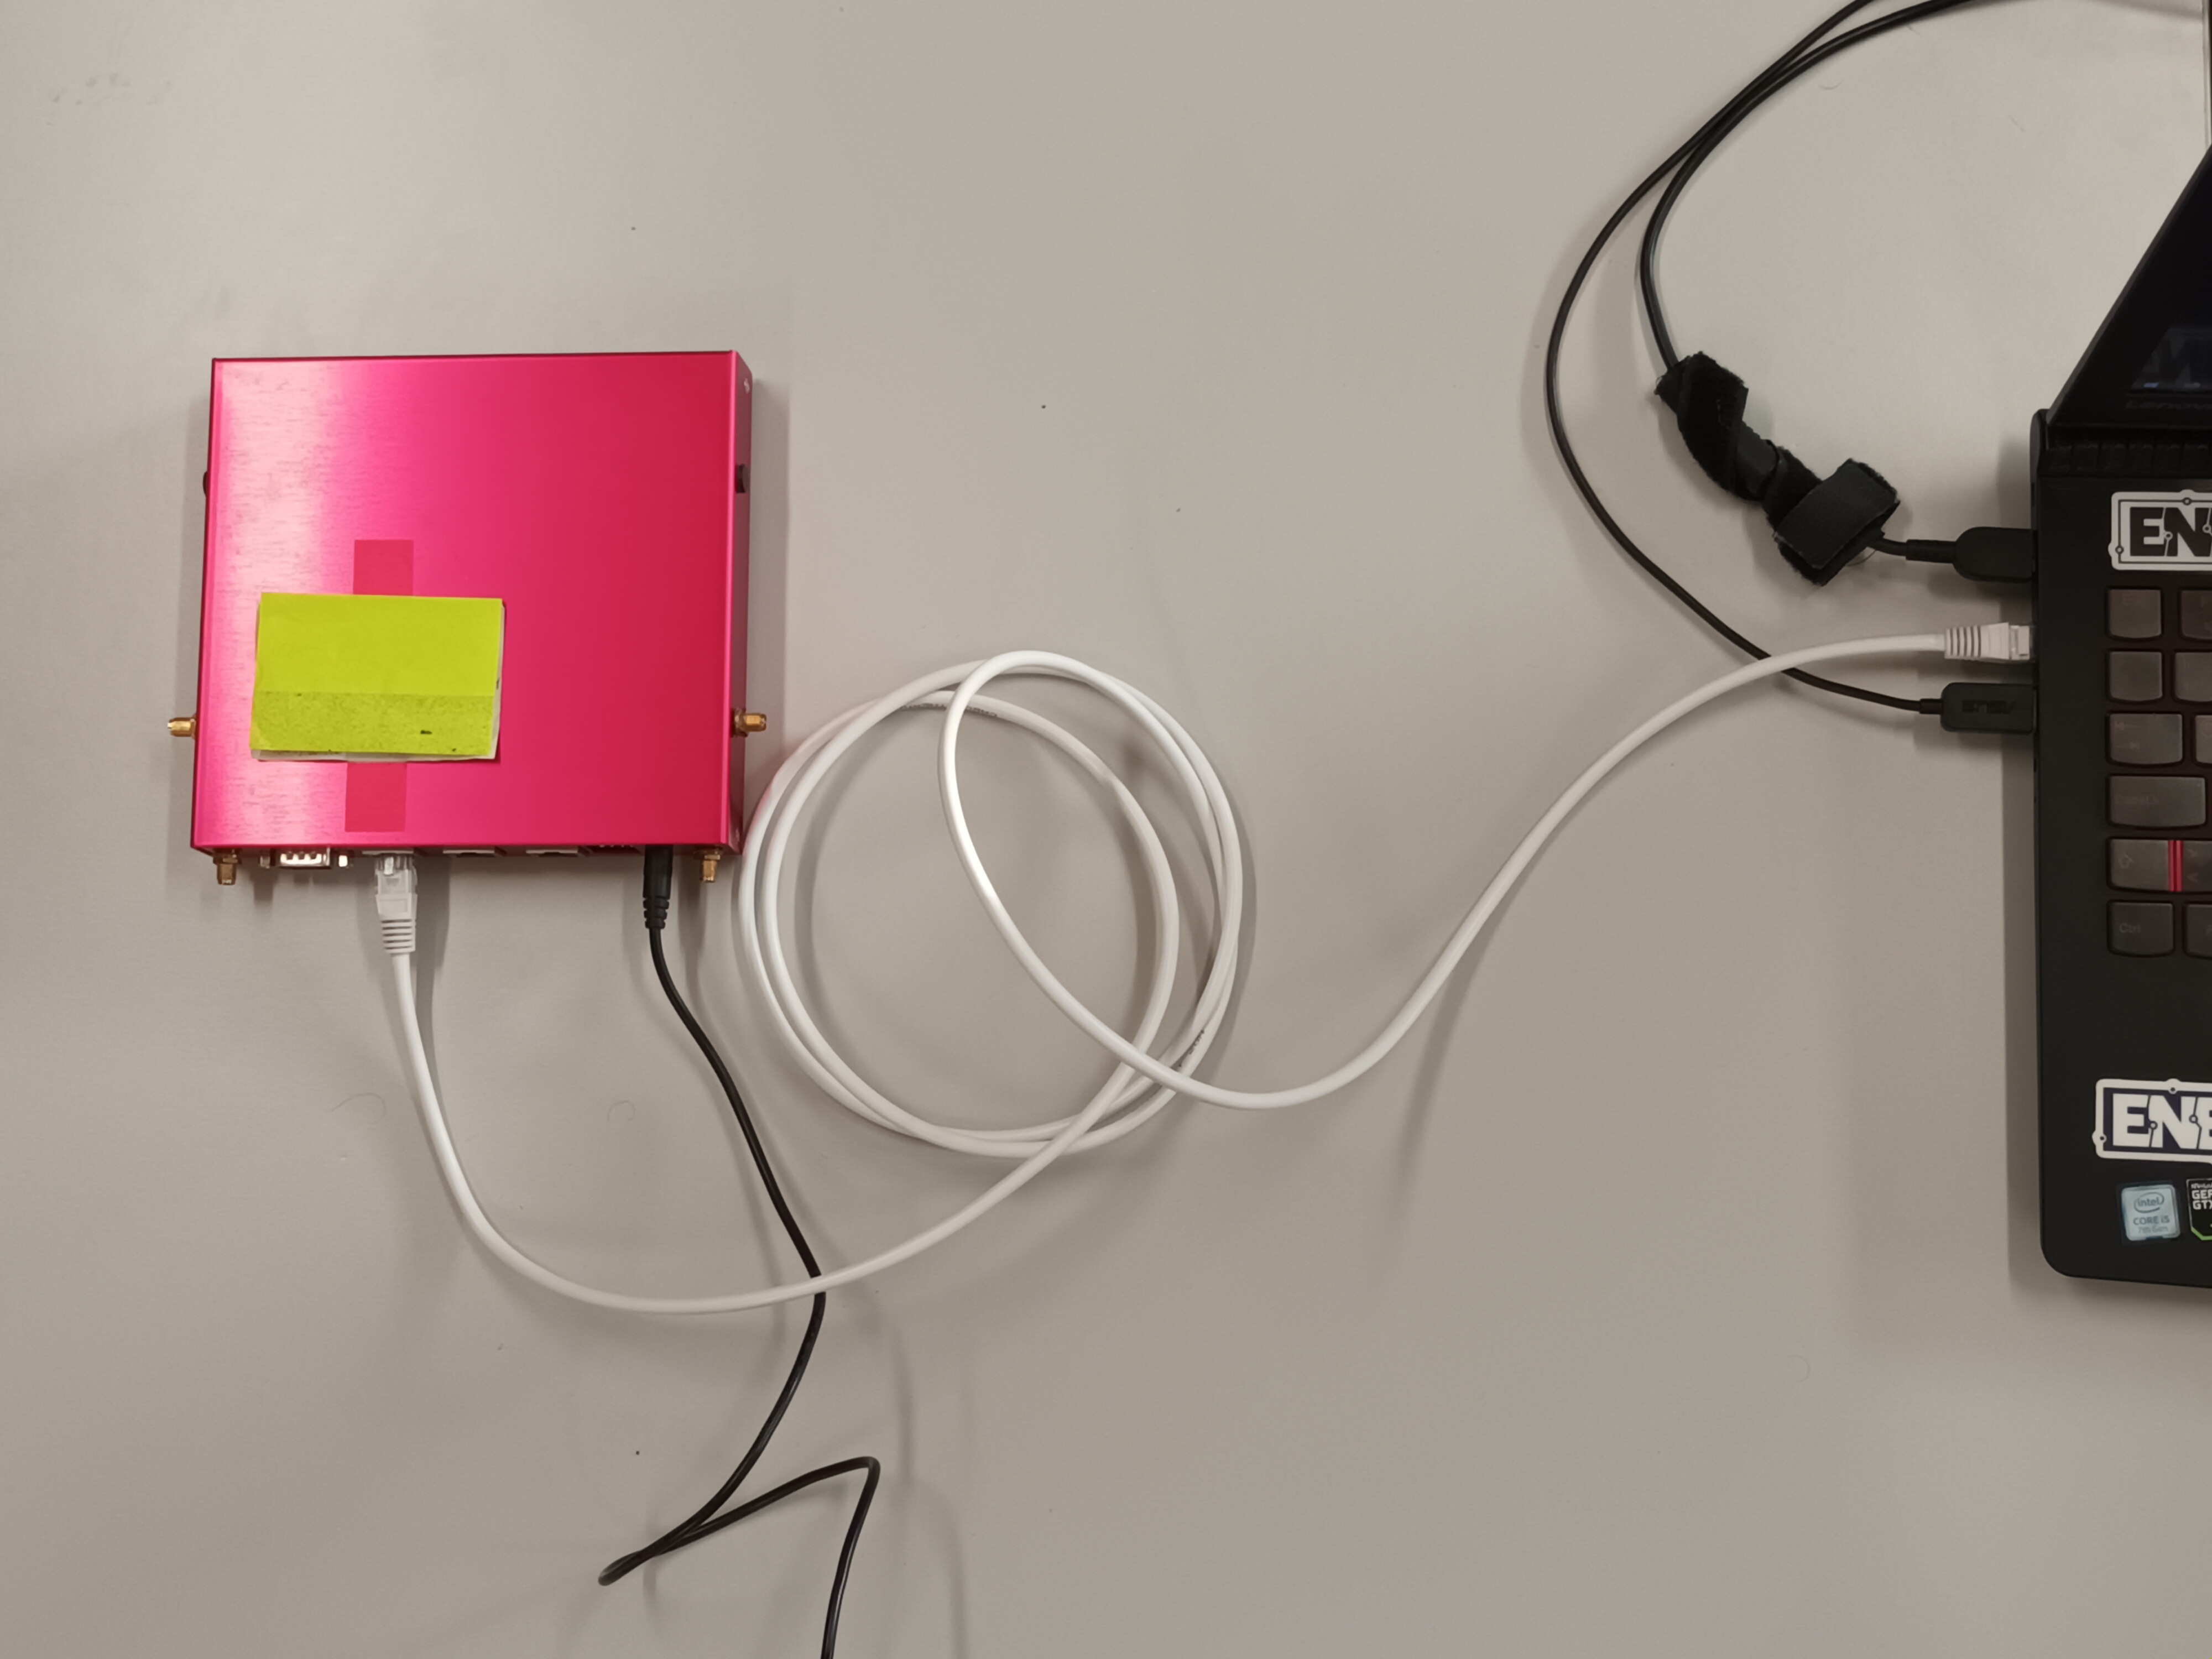
\includegraphics[width=\textwidth]{Chapters/Figures/tests/ovs_phase_1/20241122_155830.jpg}
	\caption{Setup from the first phase of the experiments with \gls{ovs}}
	\label{fig:exp1_phase1_setup}
\end{figure}

\begin{figure}
	\centering
	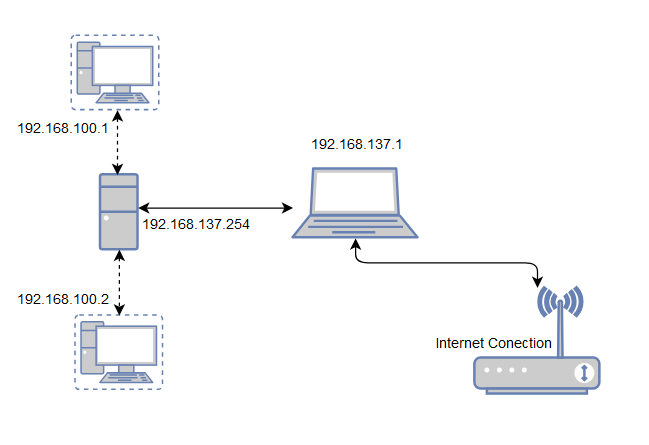
\includegraphics[width=\textwidth]{Chapters/Figures/tests/ovs_phase_1/setup_diagram.PNG}
	\caption{Diagram that represents the setup from the first phase of the experiments with \gls{ovs}}
	\label{fig:exp1_phase1_diagram}
\end{figure}

			% Results
\subsubsection{Results}

When viewed through the lens of \gls{sdn}, the configuration of this phase can be conceptualized as illustrated in Figure\ref{fig:exp1_phase1_sdn_diagram}.

\begin{figure}
	\centering
	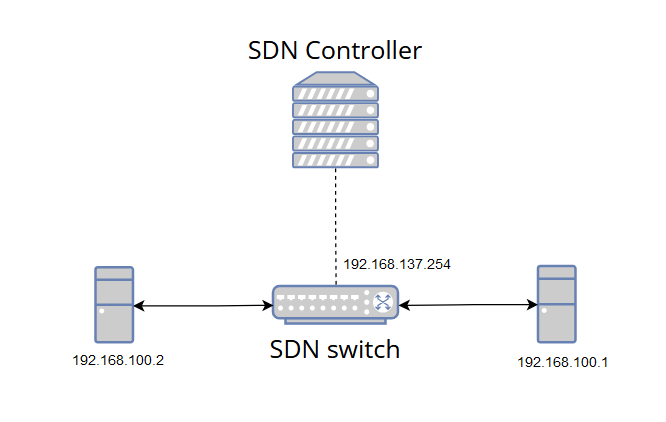
\includegraphics[width=\textwidth]{Chapters/Figures/tests/ovs_phase_1/sdn_diagram.PNG}
	\caption{Diagram that depicts the \gls{sdn} perspective of the setup from the first phase of the experiments with \gls{ovs}}
	\label{fig:exp1_phase1_sdn_diagram}
\end{figure}

The configuration of \gls{ovs}, together with information of the devices interfaces can be seen in Figure\ref{fig:exp1_phase1_ovsctl_show}.

\begin{figure}
	\centering
	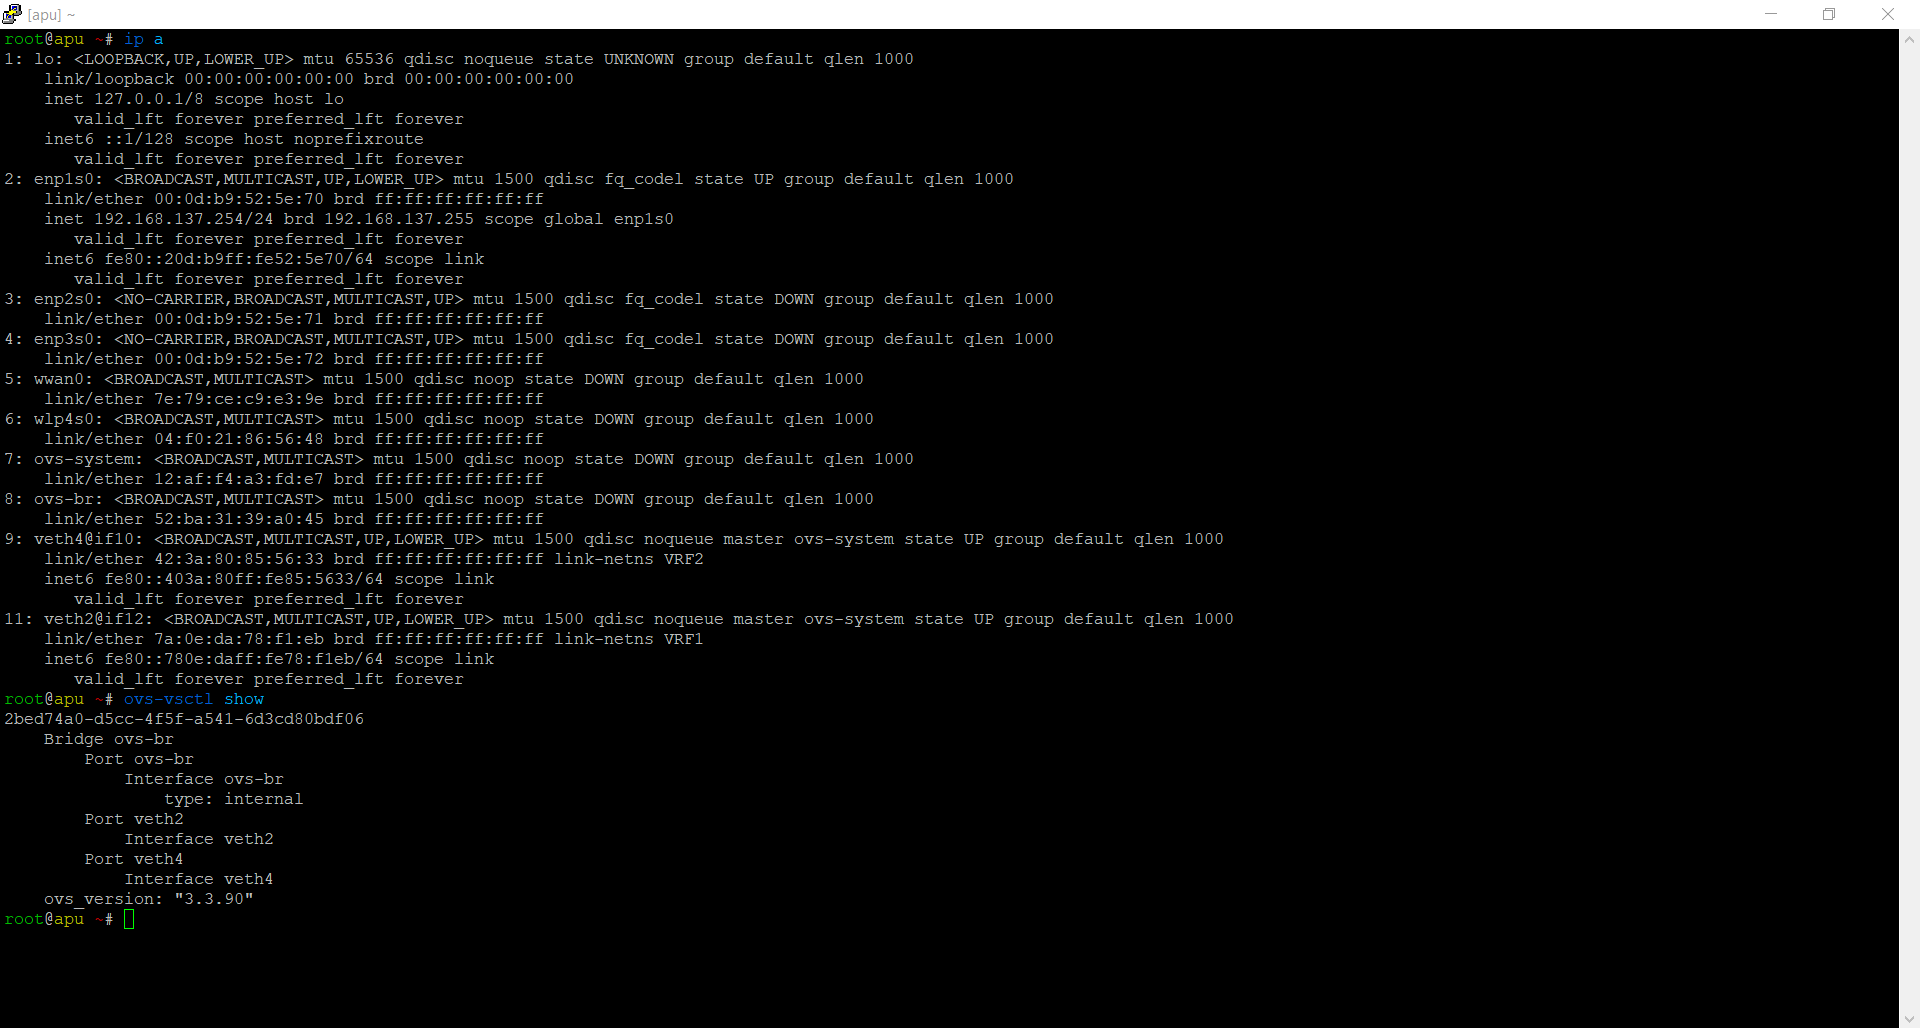
\includegraphics[width=\textwidth]{Chapters/Figures/tests/ovs_phase_1/device_ports&ovs_config.PNG}
	\caption{Results from running the commands "ip a" and "ovs-vsctl show" in the device used in phase 1\gls{ovs}}
	\label{fig:exp1_phase1_ovsctl_show}
\end{figure}

Information about the two \glspl{vrf}, as well as connectivity between them is displayed in Figure\ref{fig:exp1_phase1_pings}.

\begin{figure}
	\centering
	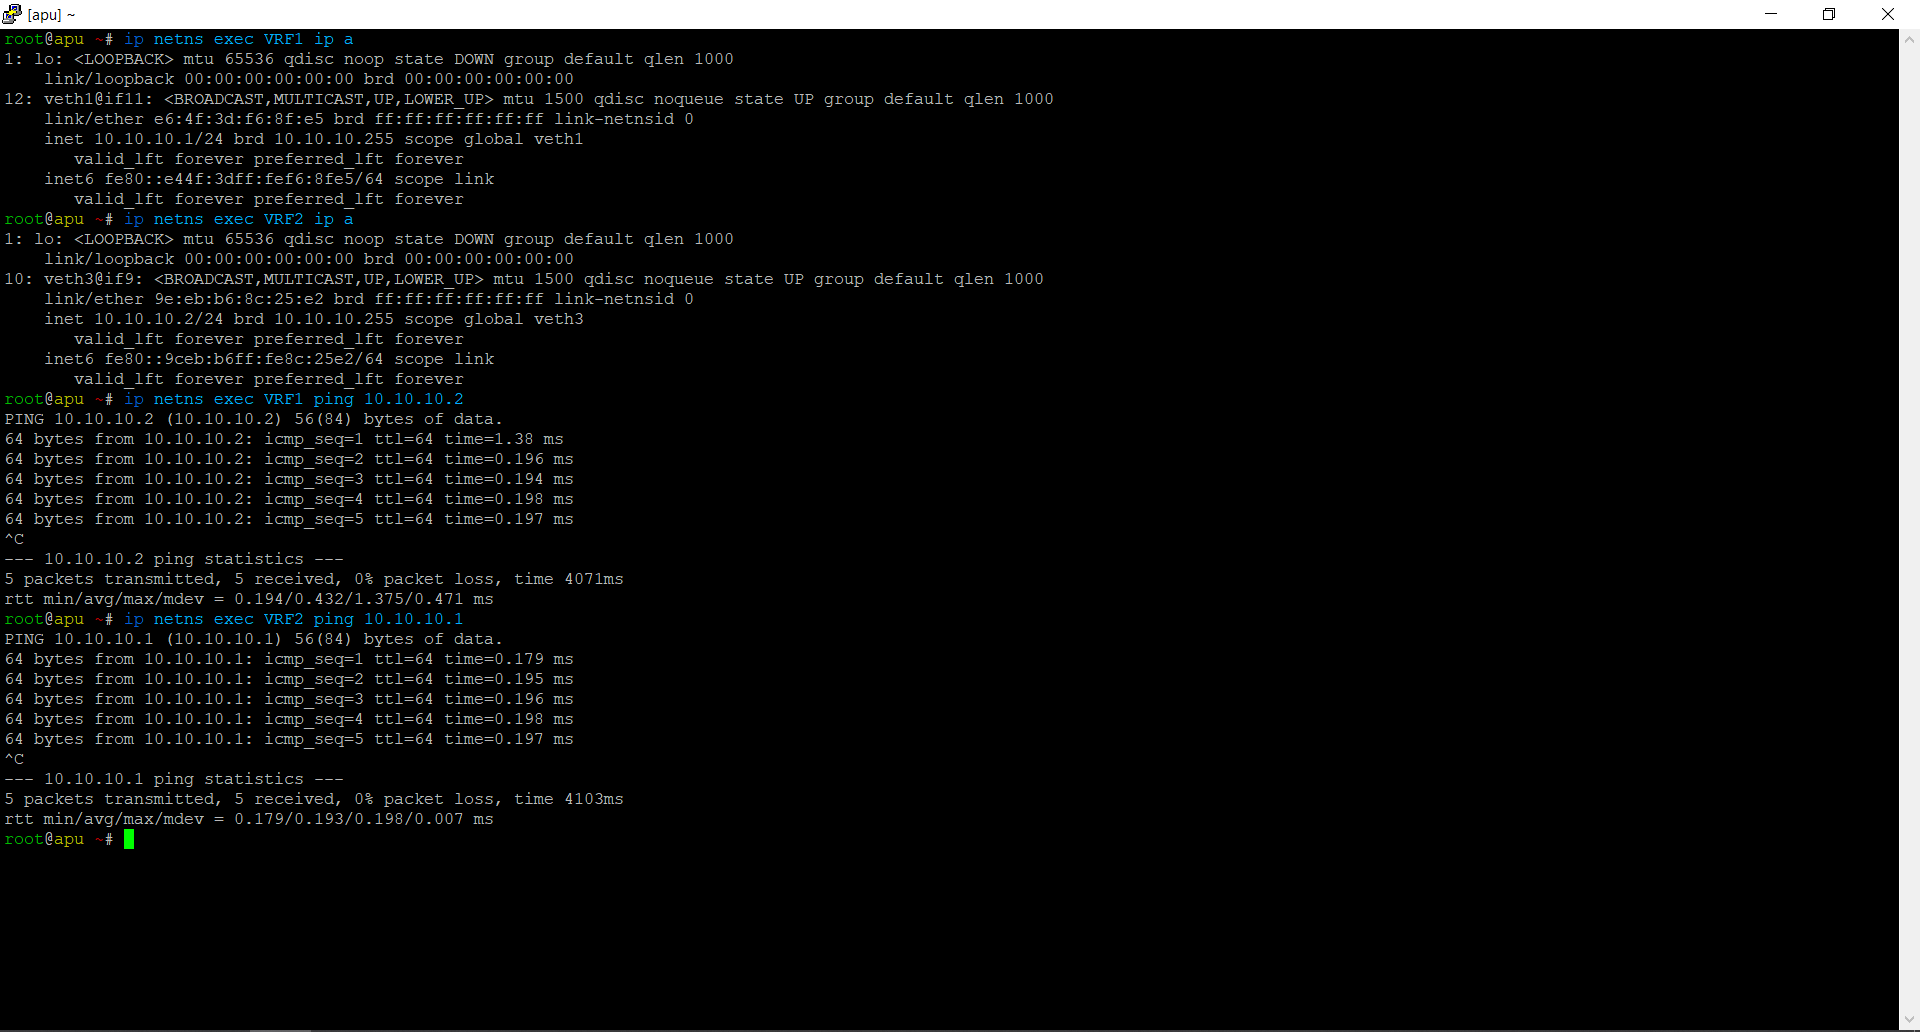
\includegraphics[width=\textwidth]{Chapters/Figures/tests/ovs_phase_1/VRF_config_&_pings.PNG}
	\caption{Results from running the commands "ip a" on both \glspl{vrf} and "ping" between them}
	\label{fig:exp1_phase1_pings}
\end{figure}


			% Phase 2
\subsection{Phase 2}
Following the success of this initial phase, the decision was made to proceed with the introduction of the remote controller. The controller, which will be utilized for the remainder of the tests, introduced an elevated level of complexity, providing an excellent opportunity to become acquainted with \gls{onos} environments. Consequently, phase two entailed the creation of a Linux-based \gls{vm} utilizing VirtualBox, with the installation of \gls{onos} on this \gls{vm}. \gls{onos} was therefore incorporated into the preceding scenario and connected to \gls{ovs} via OpenFlow.

The setup from this second phase is visualy the same as in the first phase, and can therefore be observed in Figure\ref{fig:exp1_phase1_setup}. The setup of this phase is diagrammatically represented in Figure\ref{fig:exp1_phase2_diagram}.

\begin{figure}
	\centering
	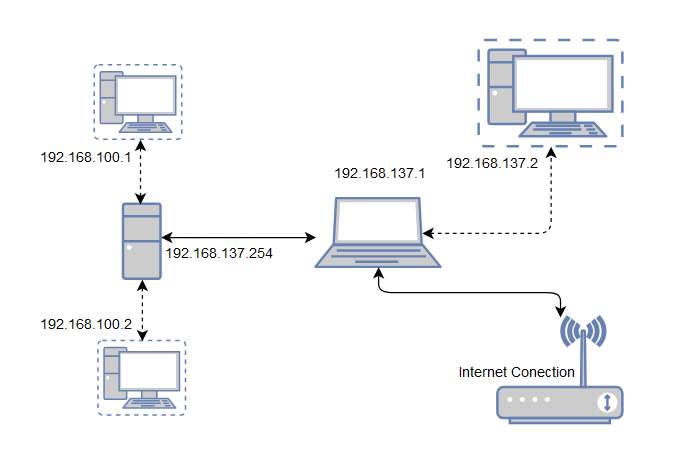
\includegraphics[width=\textwidth]{Chapters/Figures/tests/ovs_phase_2/setup_diagram.PNG}
	\caption{Diagram that represents the setup from the second phase of the experiments with \gls{ovs}}
	\label{fig:exp1_phase2_diagram}
\end{figure}

			% Results
\subsubsection{Results}

When viewed through the lens of \gls{sdn}, the configuration of this phase can be conceptualized as illustrated in Figure\ref{fig:exp1_phase2_sdn_diagram}.

\begin{figure}
	\centering
	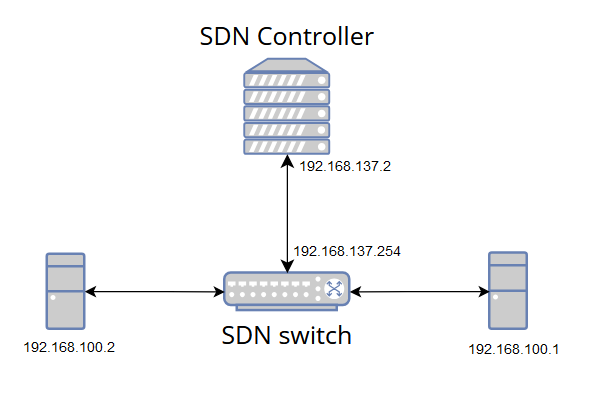
\includegraphics[width=\textwidth]{Chapters/Figures/tests/ovs_phase_2/sdn_diagram.PNG}
	\caption{Diagram that depicts the \gls{sdn} perspective of the setup from the second phase of the experiments with \gls{ovs}}
	\label{fig:exp1_phase2_sdn_diagram}
\end{figure}

The configuration of \gls{ovs}, together with showing connectivity between the two \glspl{vrf} is displayed in Figure\ref{fig:exp1_phase2_pings}.

\begin{figure}
	\centering
	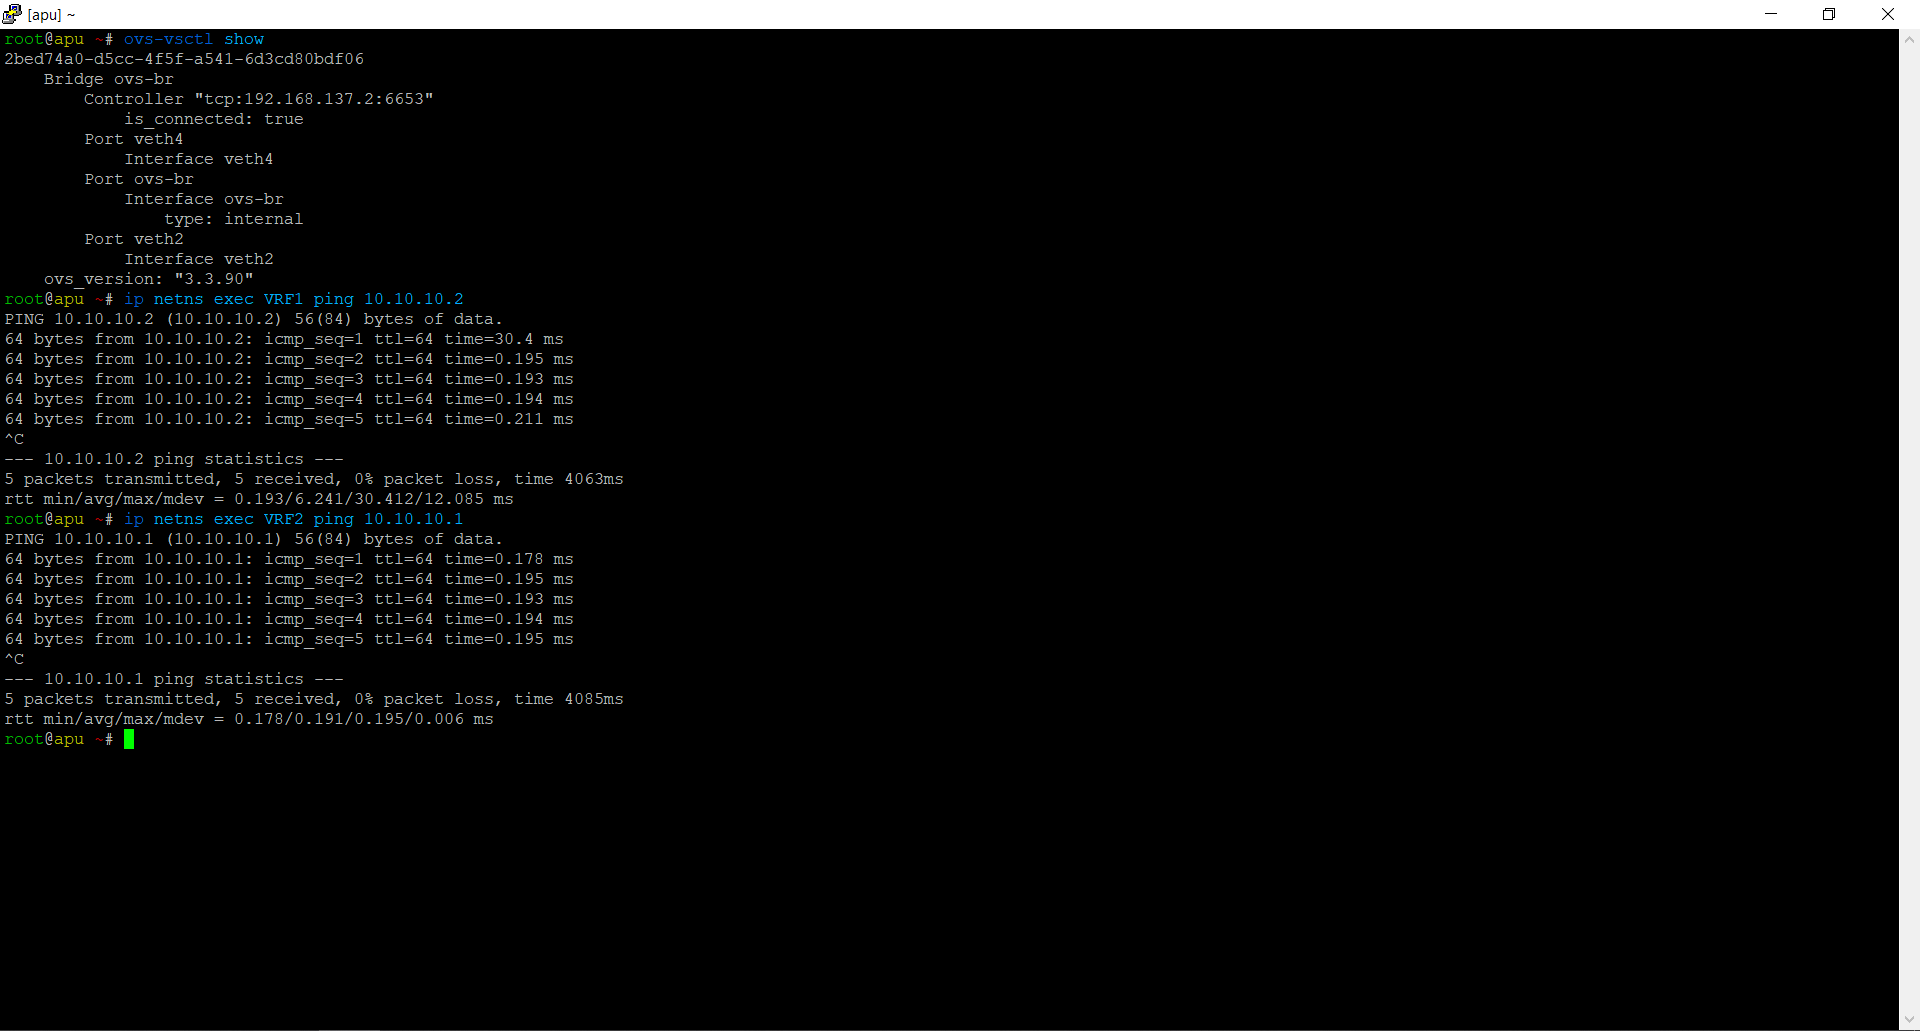
\includegraphics[width=\textwidth]{Chapters/Figures/tests/ovs_phase_2/ovs_config_&_pings.PNG}
	\caption{Results from running the commands "ovs-vsctl show" and "ping" between both \glspl{vrf}}
	\label{fig:exp1_phase2_pings}
\end{figure}

The list of devices and hosts known to the controller, along with the flows that have been injected into the devices, is presented in Figure\ref{fig:exp1_phase2_onos}.

\begin{figure}
	\centering
	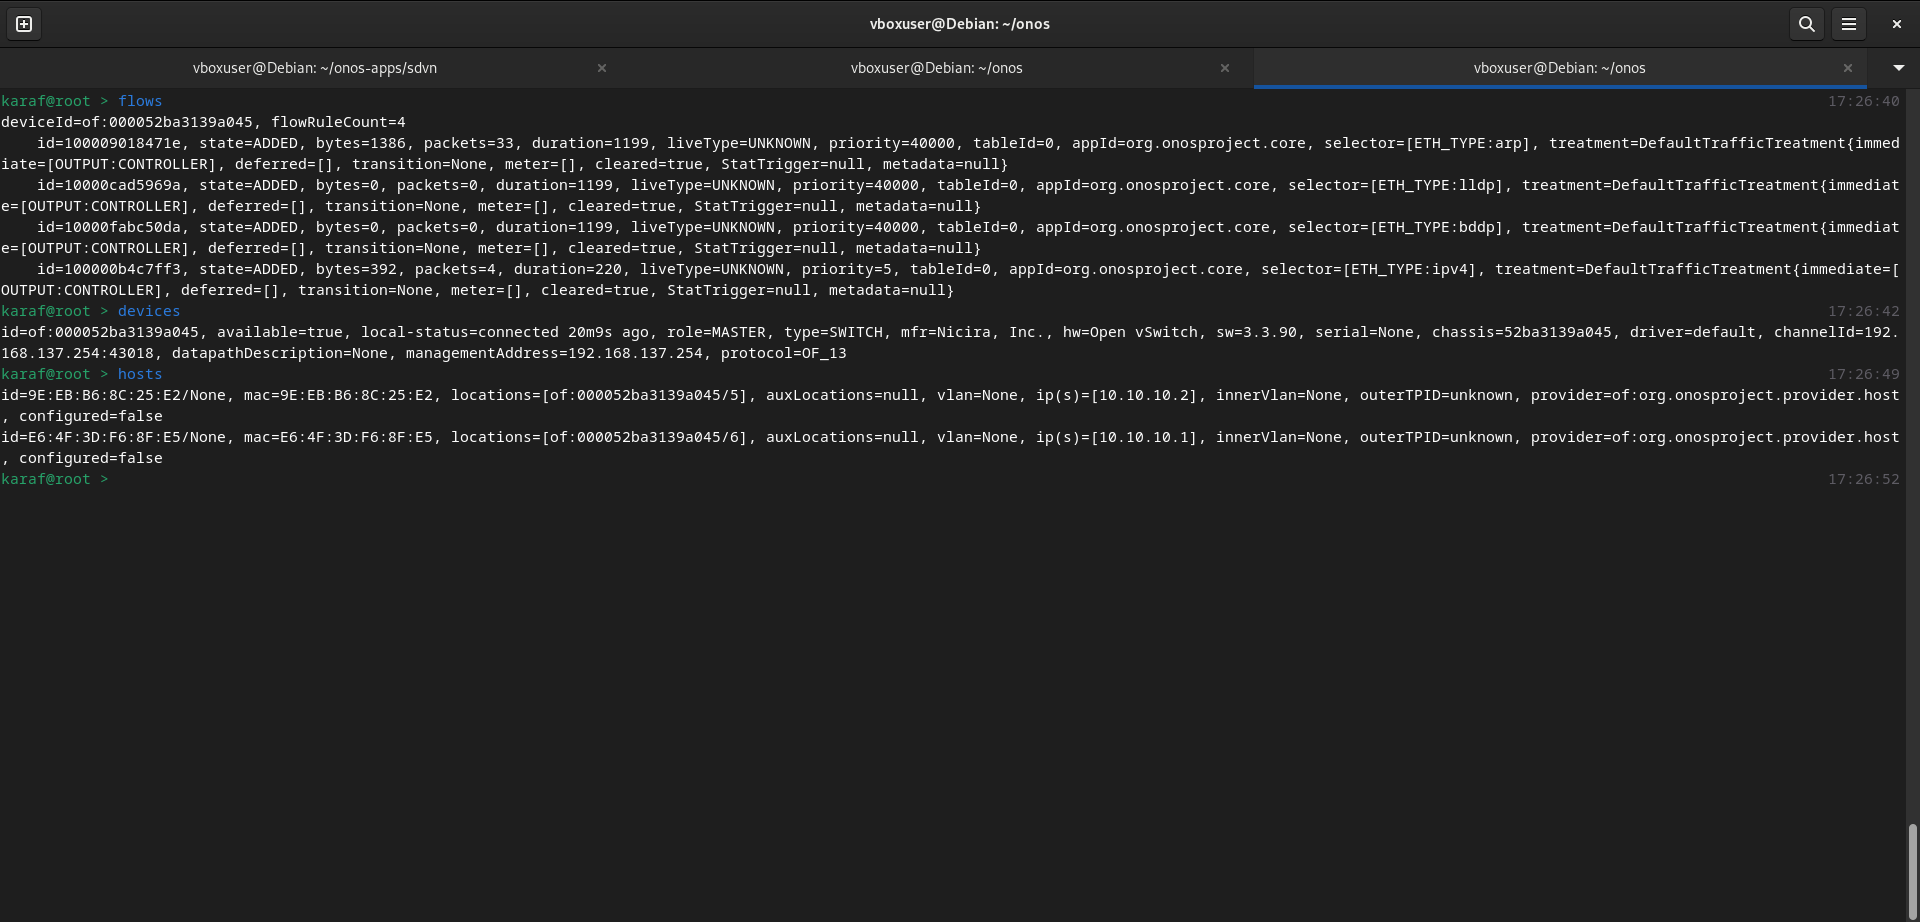
\includegraphics[width=\textwidth]{Chapters/Figures/tests/ovs_phase_2/onos_topology_&_more.PNG}
	\caption{\gls{onos} console with information relating to the devices, hosts and flows of the network}
	\label{fig:exp1_phase2_onos}
\end{figure}

			% Phase 3
\subsection{Phase 3}
By the time phase 3 was reached, the two additional devices had been received, thus enabling the substitution of the virtual interfaces with their physical counterparts. This was achieved by connecting the aforementioned two additional devices to the primary unit on which \gls{ovs} had previously been installed. The objective of this test was to verify the functionality of \gls{ovs} with non-virtual interfaces.

The setup from this third phase can be observed in Figure\ref{fig:exp1_phase3_setup}. The setup of this phase is diagrammatically represented in Figure\ref{fig:exp1_phase3_diagram}.

\begin{figure}
	\centering
	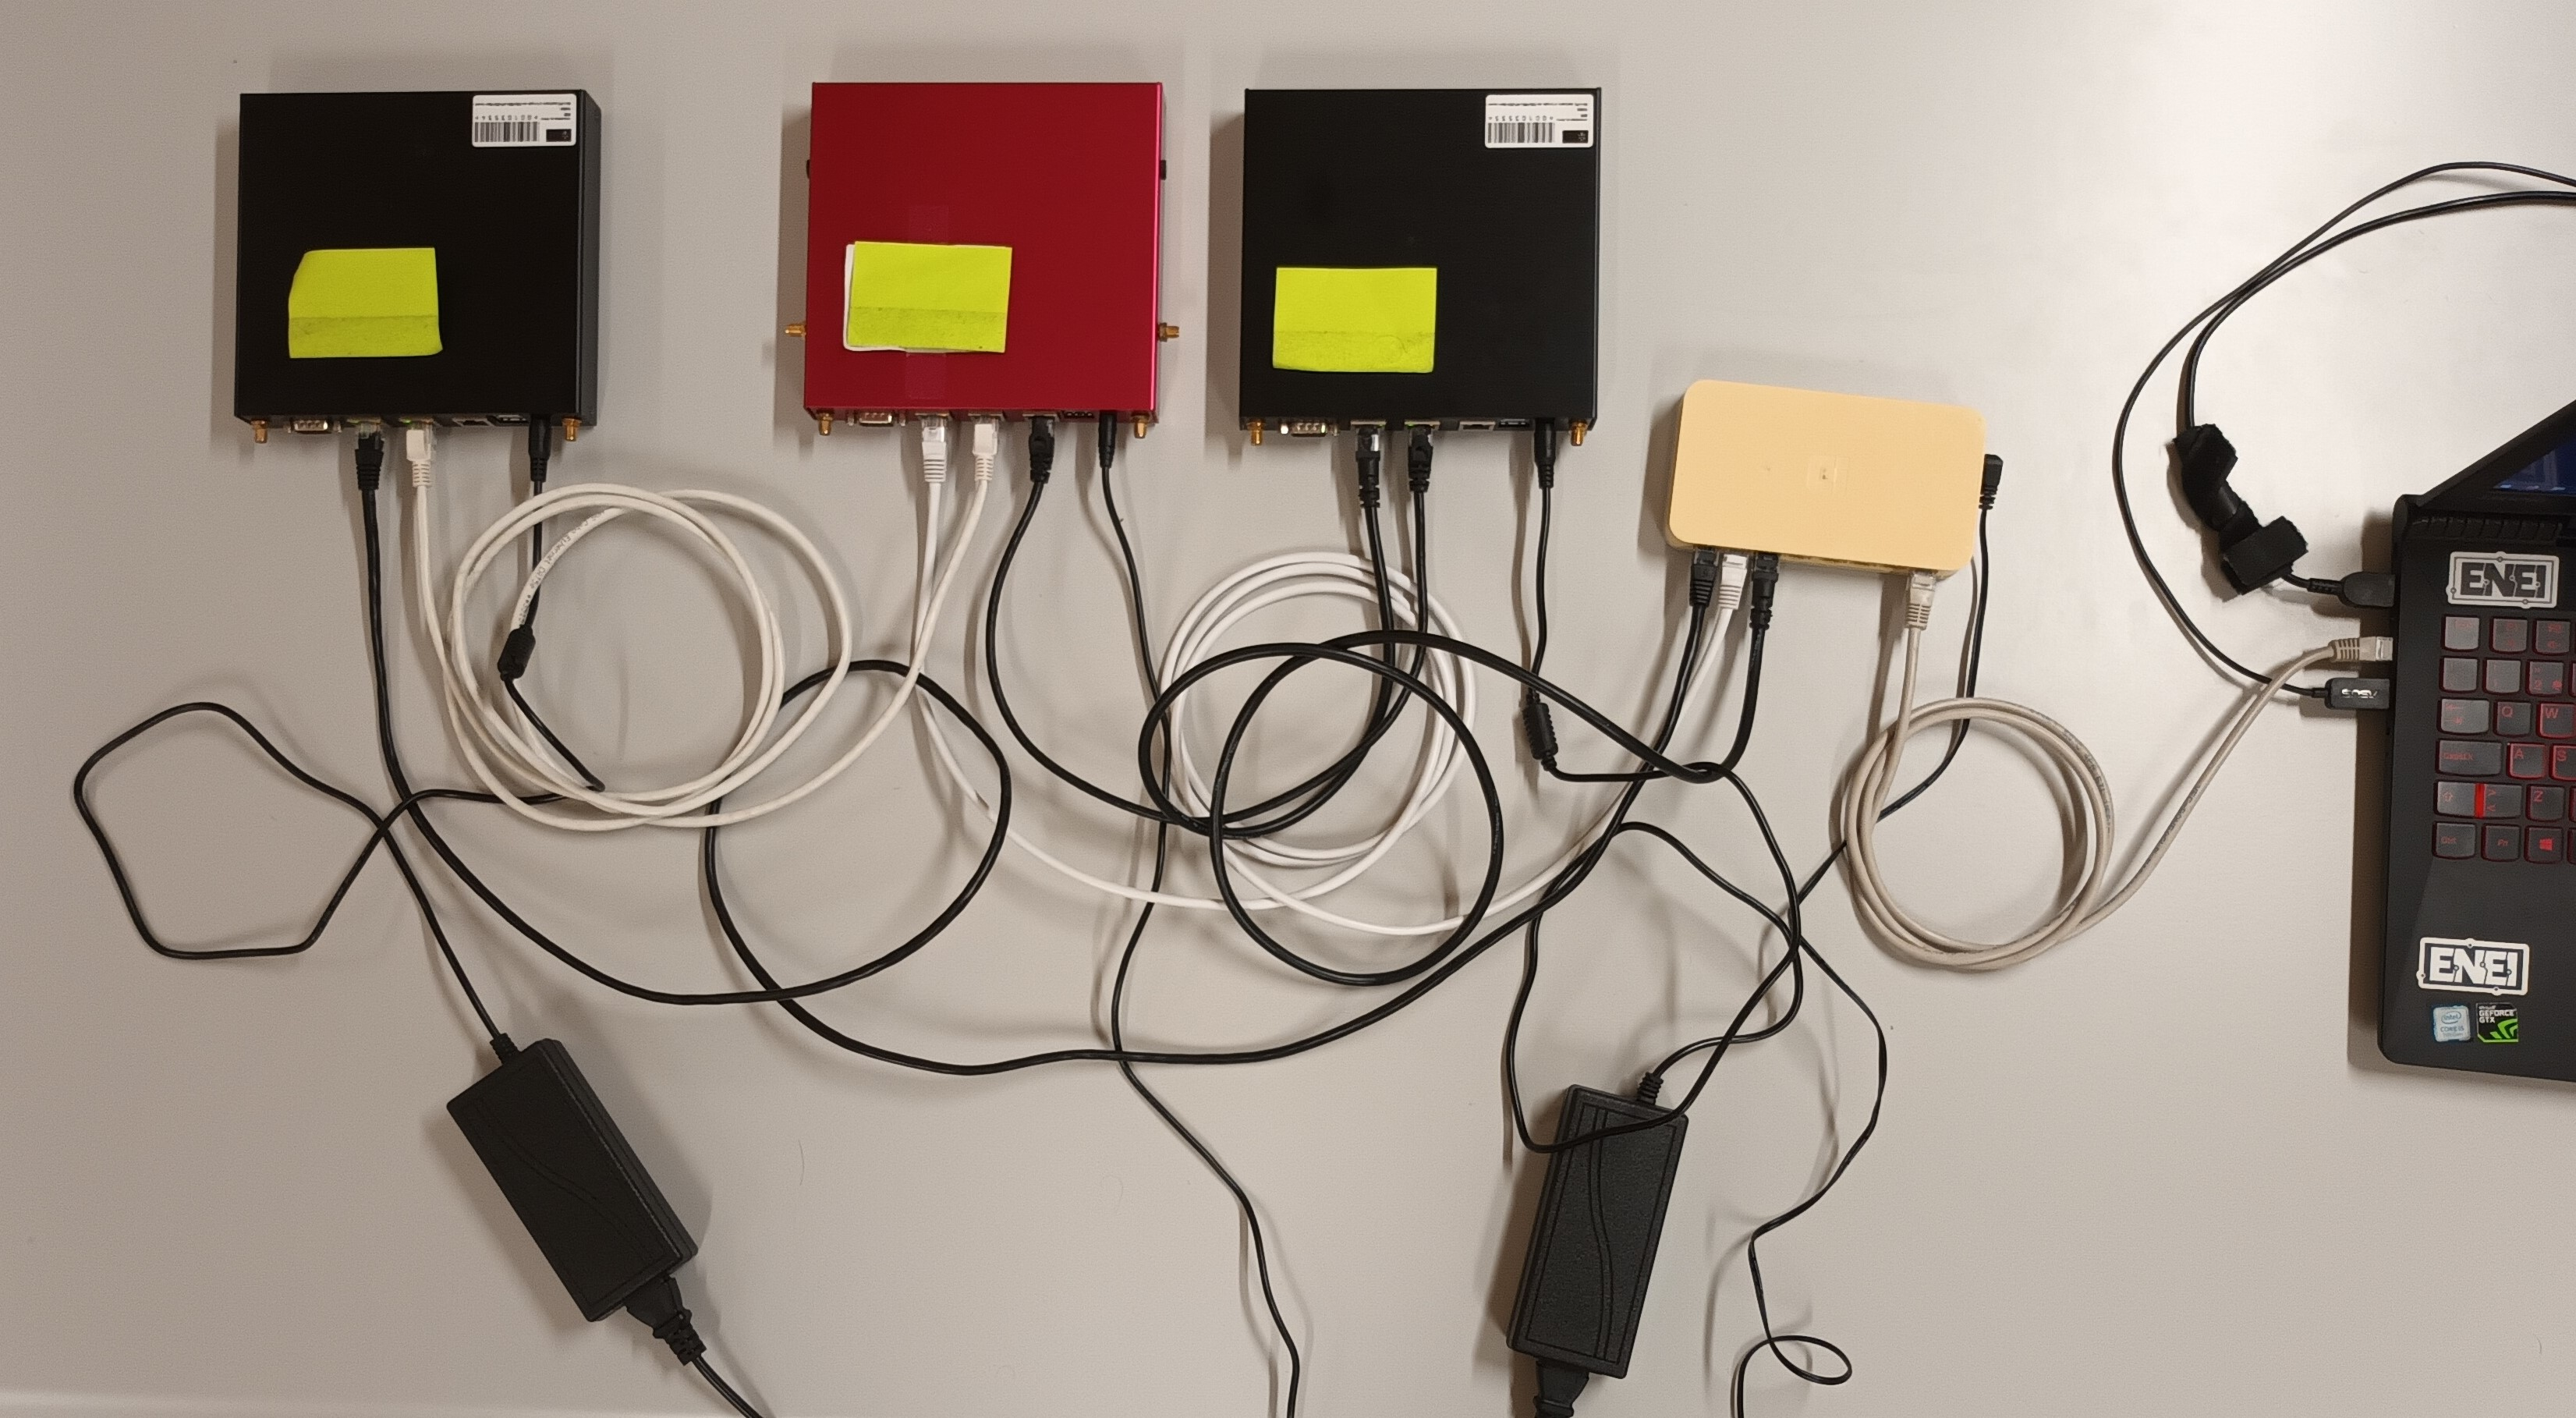
\includegraphics[width=\textwidth]{Chapters/Figures/tests/ovs_phase_3/setup.jpg}
	\caption{Setup from the third phase of the experiments with \gls{ovs}}
	\label{fig:exp1_phase3_setup}
\end{figure}

\begin{figure}
	\centering
	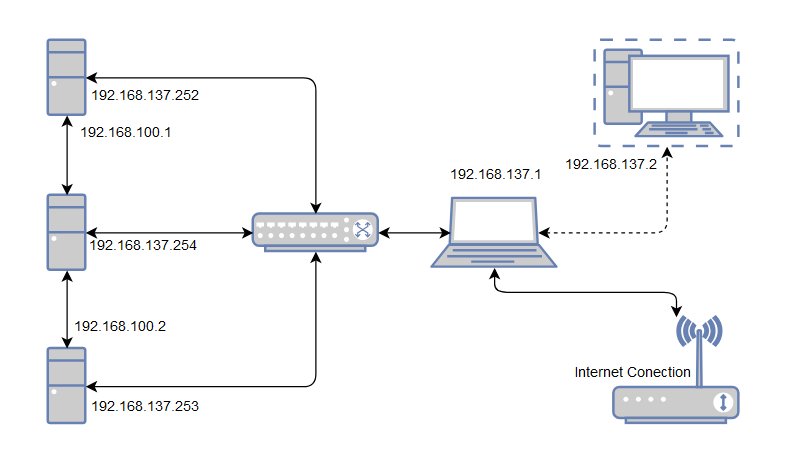
\includegraphics[width=\textwidth]{Chapters/Figures/tests/ovs_phase_3/setup_diagram.PNG}
	\caption{Diagram that represents the setup from the third phase of the experiments with \gls{ovs}}
	\label{fig:exp1_phase3_diagram}
\end{figure}

			% Results
\subsubsection{Results}

From the perspective of \gls{sdn}, the network configuration of this phase is identical to that of the previous phase. Consequently, it can be observed in Figure\ref{fig:exp1_phase2_sdn_diagram}.

The configuration of \gls{ovs}, together with showing connectivity between the two other devices is displayed in Figure\ref{fig:exp1_phase3_pings}.

\begin{figure}
	\centering
	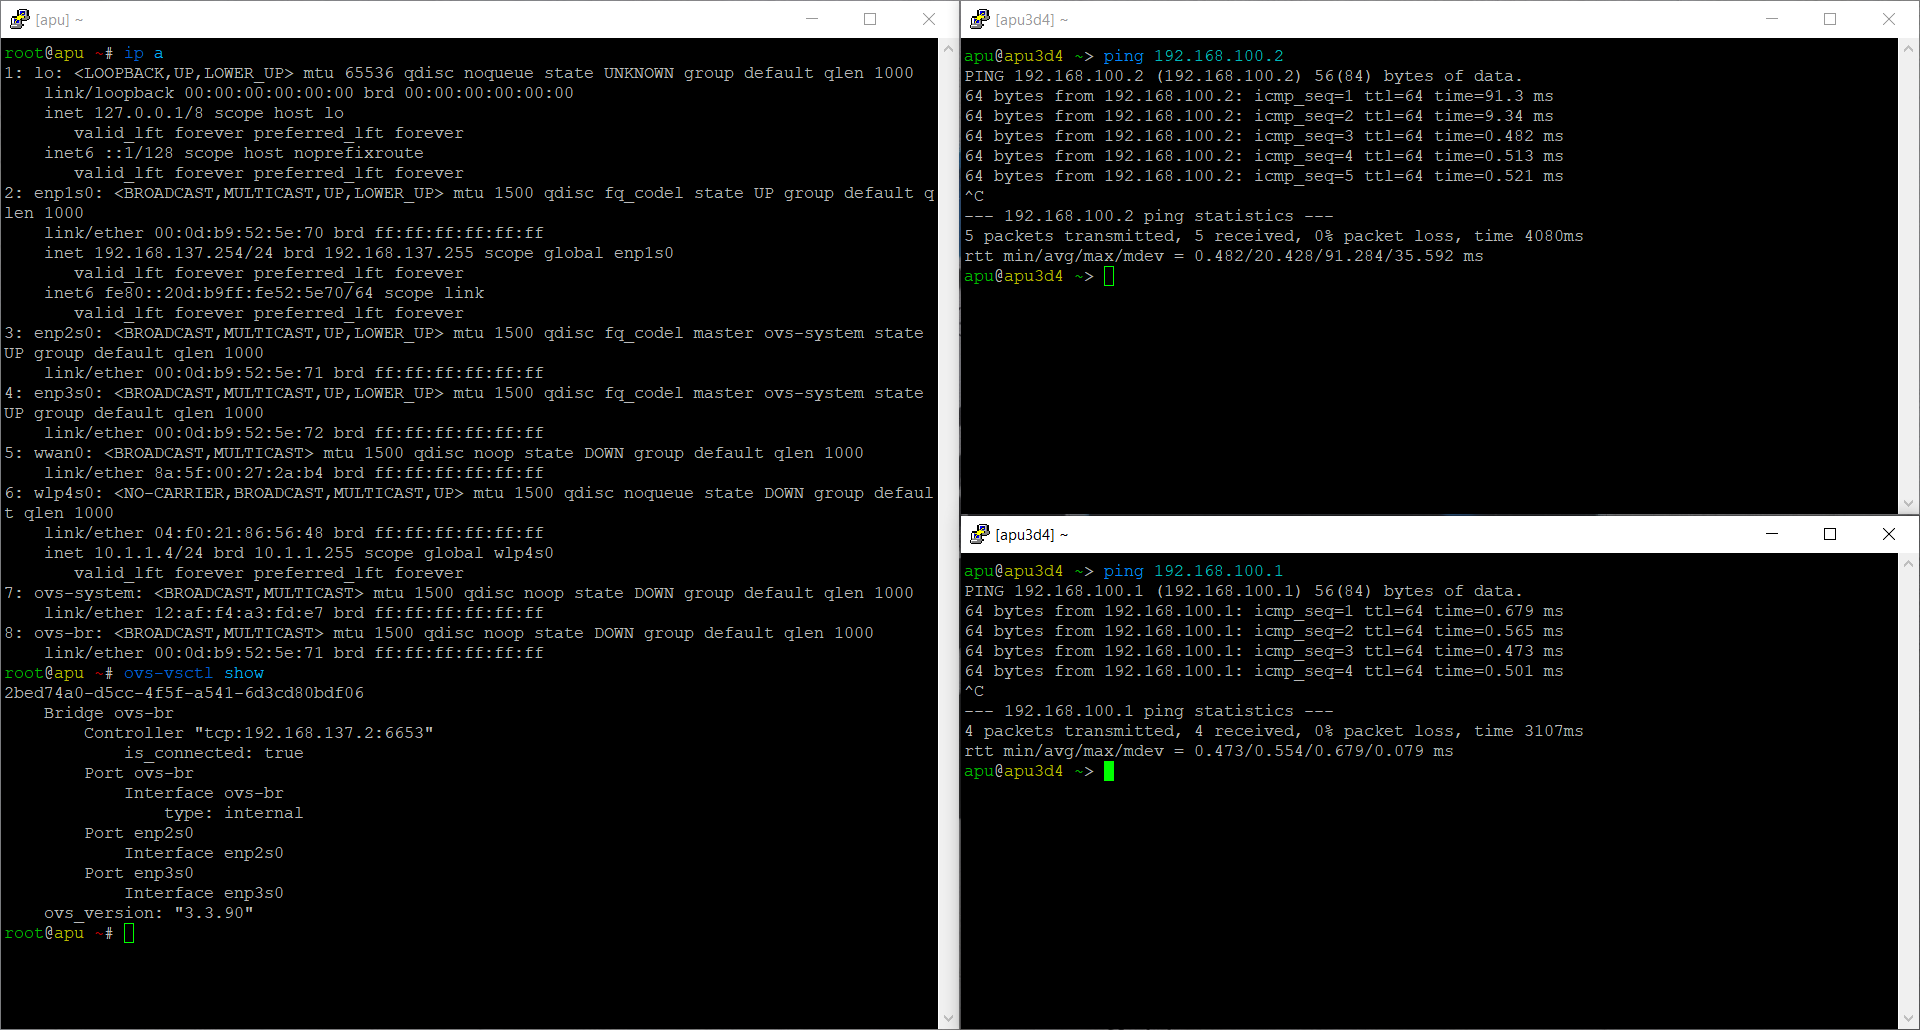
\includegraphics[width=\textwidth]{Chapters/Figures/tests/ovs_phase_3/ovs_config_&_pings.PNG}
	\caption{Results from running the commands "ip a" and "ovs-vsctl show" on the device running \gls{ovs} and "ping" between the other two devices}
	\label{fig:exp1_phase3_pings}
\end{figure}

The list of devices and hosts known to the controller, along with the flows that have been injected into the devices, is presented in Figure\ref{fig:exp1_phase3_onos}.

\begin{figure}
	\centering
	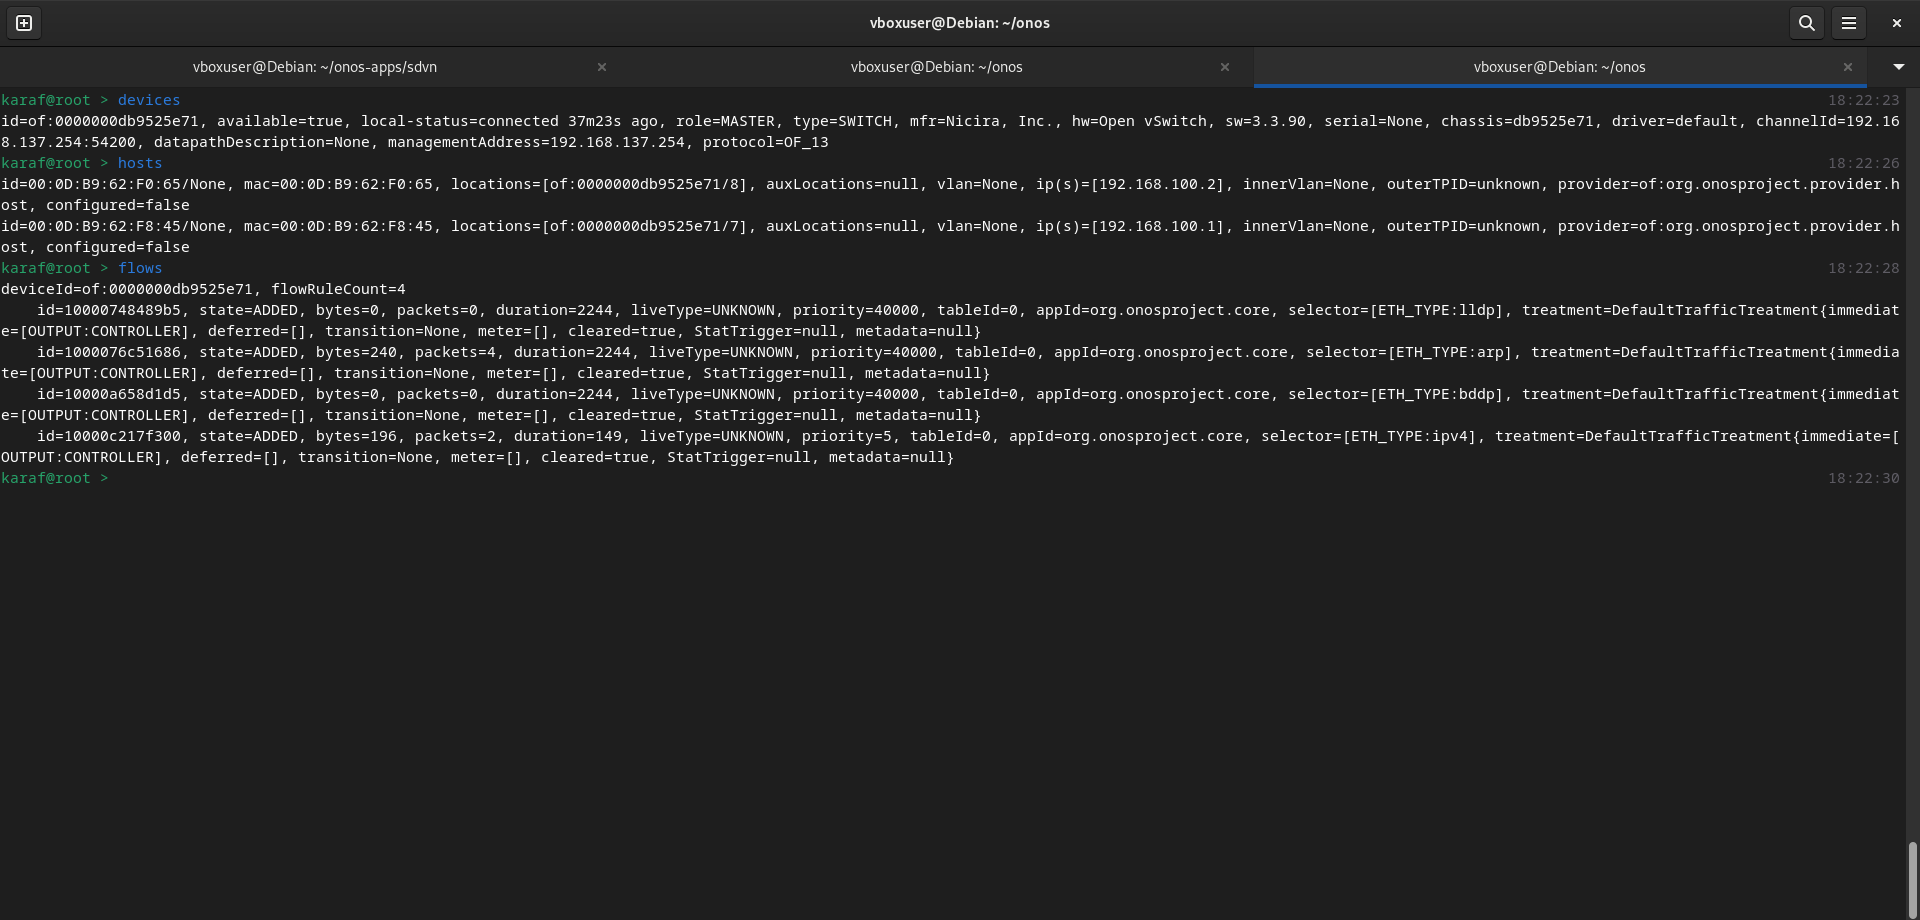
\includegraphics[width=\textwidth]{Chapters/Figures/tests/ovs_phase_3/onos_topology_&_config.PNG}
	\caption{\gls{onos} console with information relating to the devices, hosts and flows of the network}
	\label{fig:exp1_phase3_onos}
\end{figure}

			% Phase 4
\subsection{Phase 4}
In Phase 4, the test \gls{sdn} network was expanded to integrate the three devices by installing \gls{ovs} on the two new devices. Consequently, the three devices were linked together and connected to the \gls{onos} controller, and two \glspl{vrf} were created, each situated on opposite edges of the network. 


This configuration is equal to the last phase, so it is illustrated in Figure \ref{fig:exp1_phase3_setup}. The setup of this phase is diagrammatically represented in Figure\ref{fig:exp1_phase4_diagram} and described in the following itemized list:

\begin{itemize}
	\item 192.168.137.1 - This \gls{ip} address identifies the author's personal laptop computer. It serves as the central coordinating hub for the entire network, facilitating the observation and monitoring of all network activity.
	\item 192.168.137.2 - This address represents a virtual machine that is hosted on the author's laptop via the Oracle VM VirtualBox virtualization platform. The virtual environment is configured with Debian 12 and is primarily intended for the deployment of \gls{onos}. This configuration is essential due to the fact that the primary branch of \gls{onos} is designed to run on Linux, whereas the author's device runs on Windows.
	\item 192.168.137.252 - This corresponds to a device 2. It has a fresh installation of the Ubuntu Server operating system and is running \gls{ovs}.
	\item 192.168.137.253 - This device is virtually identical to the device 192.168.137.252.
	\item 192.168.137.254 - This address represents device 1.0 that was received from the university. This device has debian 12 and is running \gls{ovs}.
	\item 10.10.10.1 - This \gls{ip} address identifies the virtual interface that has been added to the \gls{vrf} instance created in the 192.168.137.252 device.
	\item 10.10.10.2 - Identically to the last one, this \gls{ip} address identifies the virtual interface that has been added to the \gls{vrf} instance created in the 192.168.137.253 device.
\end{itemize}

\begin{figure}
	\centering
	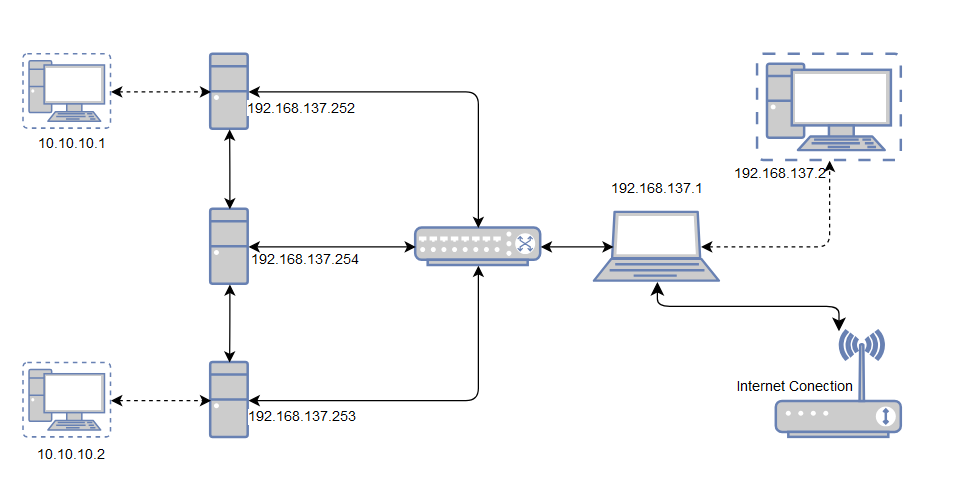
\includegraphics[width=\textwidth]{Chapters/Figures/tests/ovs_phase_4/setup_diagram.PNG}
	\caption{Diagram that represents the setup from the fourth phase of the experiments with \gls{ovs}}
	\label{fig:exp1_phase4_diagram}
\end{figure}

			% Results
\subsubsection{Results}

When viewed through the lens of \gls{sdn}, the configuration of this phase can be conceptualized as illustrated in Figure\ref{fig:exp1_phase4_sdn_diagram}.

\begin{figure}
	\centering
	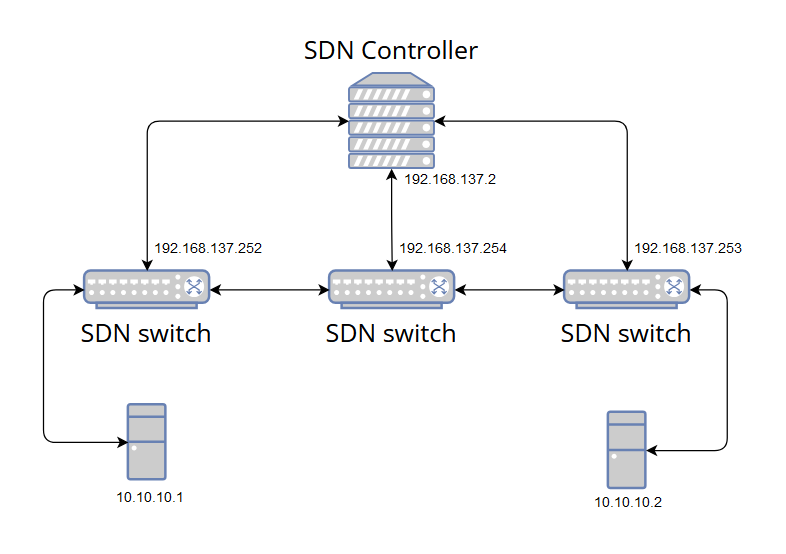
\includegraphics[width=\textwidth]{Chapters/Figures/tests/ovs_phase_4/sdn_diagram.PNG}
	\caption{Diagram that depicts the \gls{sdn} perspective of the setup from the fourth phase of the experiments with \gls{ovs}}
	\label{fig:exp1_phase4_sdn_diagram}
\end{figure}

The configuration of the three instances of \gls{ovs} that are running is Figure\ref{fig:exp1_phase4_config}.

\begin{figure}
	\centering
	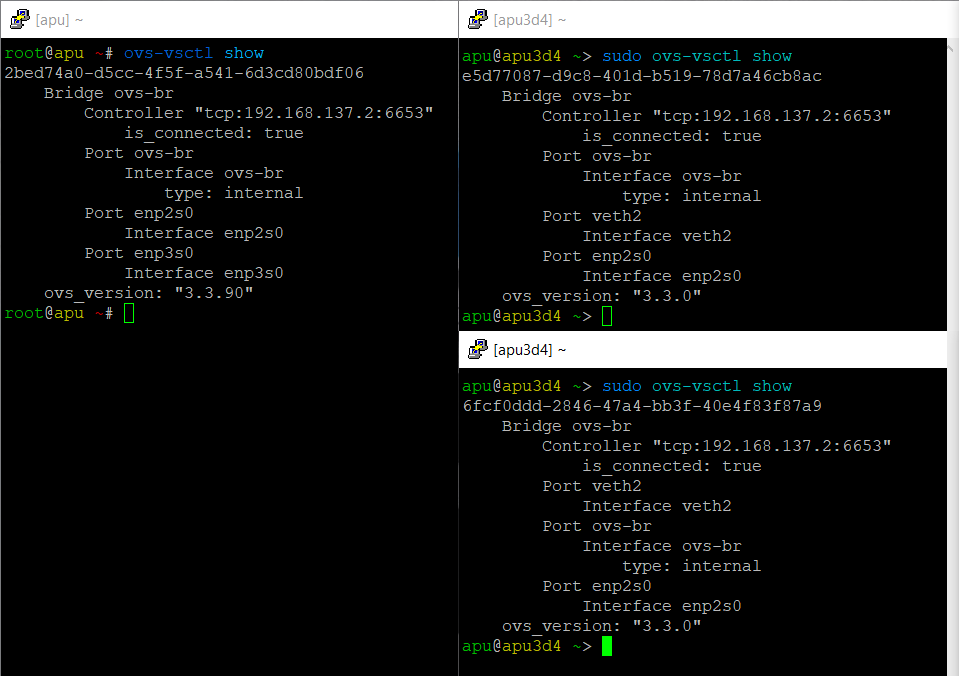
\includegraphics[width=\textwidth]{Chapters/Figures/tests/ovs_phase_4/ovs_config.PNG}
	\caption{Results from running the commands "ovs-vsctl show" in the devices running \gls{ovs}}
	\label{fig:exp1_phase4_config}
\end{figure}

Connectivity between the two \gls{vrf} is demonstraded in Figure\ref{fig:exp1_phase4_pings}. It illustrates the connectivity between devices 192.168.137.252 and 192.168.137.253, manifesting through the VFRs with \glspl{ip} 10.10.10.1 and 10.10.10.2.

\begin{figure}
	\centering
	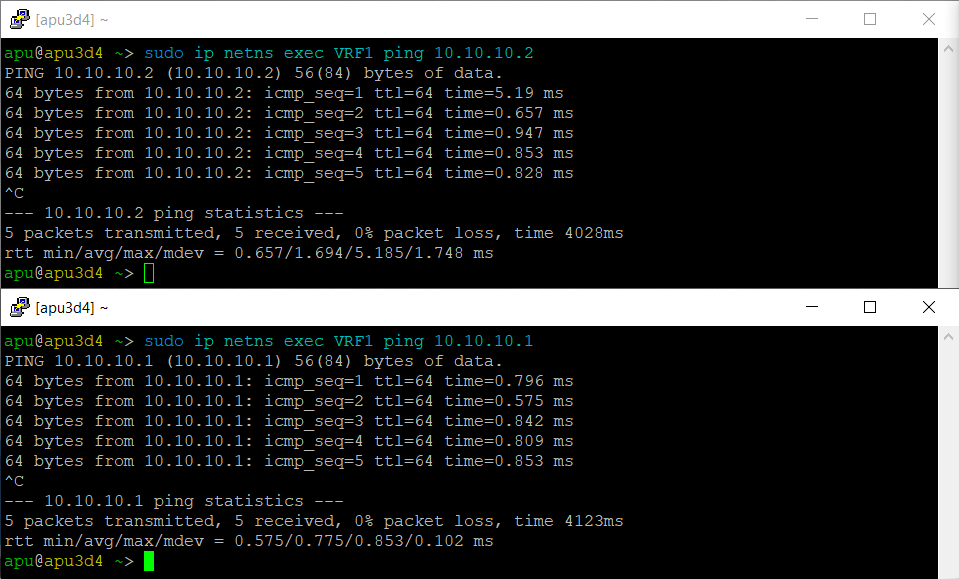
\includegraphics[width=\textwidth]{Chapters/Figures/tests/ovs_phase_4/pings.PNG}
	\caption{Results from running the commands "ping" in the \gls{vrf} between the two devices on the edge of the network}
	\label{fig:exp1_phase4_pings}
\end{figure}

The list of devices and hosts known to the controller is shown in Figure\ref{fig:exp1_phase4_onos}, and the flows that have been injected into the devices are presented in Figure\ref{fig:exp1_phase4_onos_flows}.

\begin{figure}
	\centering
	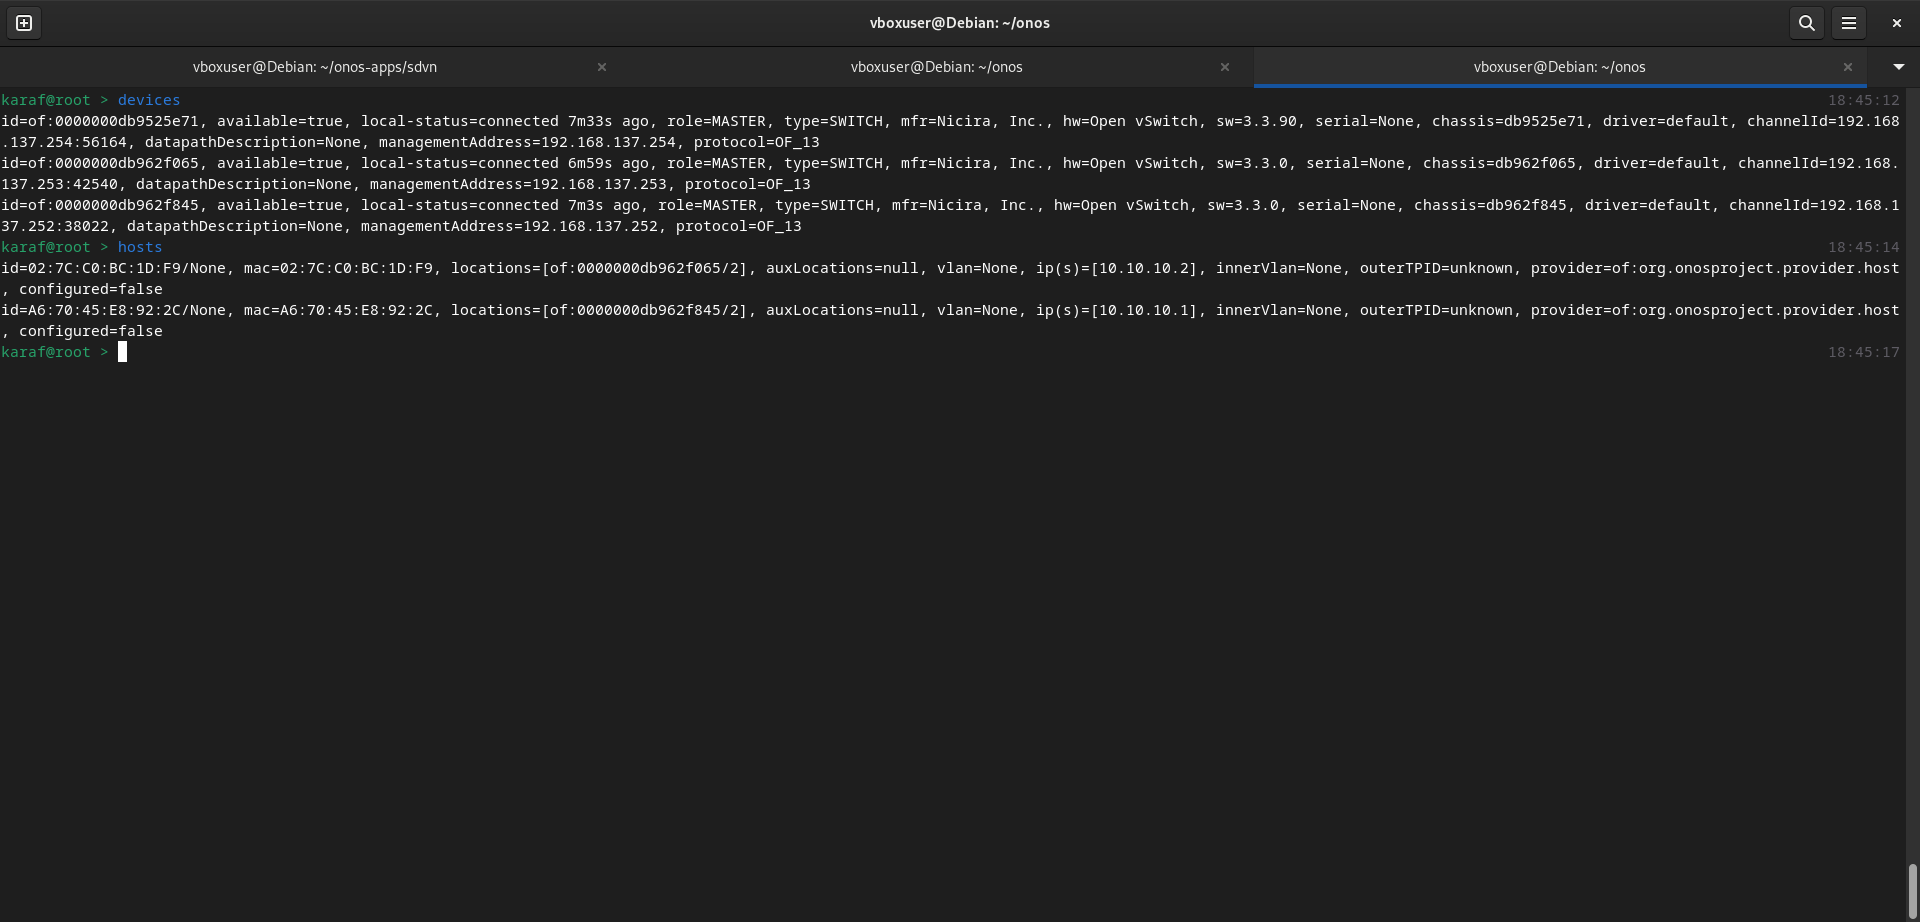
\includegraphics[width=\textwidth]{Chapters/Figures/tests/ovs_phase_4/onos_topology.PNG}
	\caption{\gls{onos} console with information relating to the devices and hosts of the network}
	\label{fig:exp1_phase4_onos}
\end{figure}

\begin{figure}
	\centering
	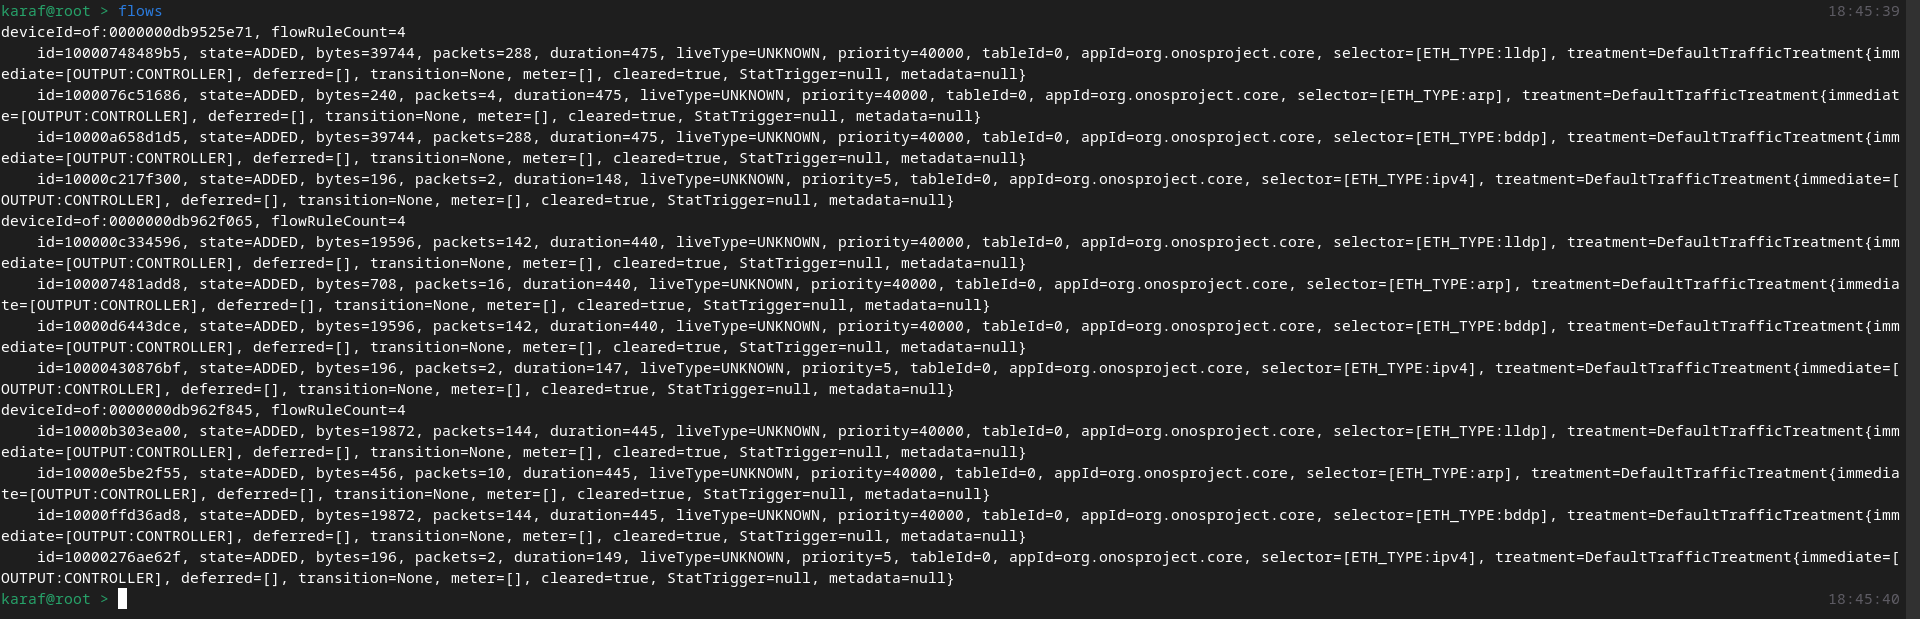
\includegraphics[width=\textwidth]{Chapters/Figures/tests/ovs_phase_4/onos_flows.PNG}
	\caption{\gls{onos} console with information relating to the flows of the network}
	\label{fig:exp1_phase4_onos_flows}
\end{figure}

 		% Analysis and Interpretation
\subsection{Analysis and Interpretation}
It was intended for the subsequent phase of the investigation to involve an attempt to introduce the ath9k patch and wireless antennas for use in conjunction with the \gls{ovs} system. However, Phase 4 proved to be the final phase of the investigation. Through additional research it was discovered that \gls{ovs} is unable to function with wireless interfaces, which was is corroborated by a statement on the official wiki\cite{noauthor_common_nodate} indicating that \gls{ovs} is not compatible with wireless interfaces.
Furthermore, the testing phase revealed another significant limitation in the capabilities of \gls{ovs}. Despite its compatibility with OpenFlow, \gls{ovs} is constrained by the traditional definition of a switch, thereby limiting its functionality to layer 2. This inherent restriction disables the system from parsing packets from different subnets.
In conclusion, it was demonstrated that the use of \gls{ovs} is not viable within the context of vehicular scenarios. These findings served to reinforce the hypothesis that OpenFlow-based solutions are not a viable option for use in vehicular environments. As anticipated and corroborated in Section\ref{cha:conceptual_solution}, OpenFlow is only compatible with traditional software protocols, thereby precluding the use of vehicular protocols under the circumstances presented here. 

% BMv2
\section[BMv2]{\gls{bmv2}}
% Test Scenarios
The objective of this experiment is to evaluate the compatibility and practicality of integrating \gls{bmv2} and \gls{p4} with \gls{vanet} technologies. The experiments were conducted using two 2-box apparatuses.

% Phase 1
\subsection{Phase 1}
Phase 1 of this experiment will focus on assessing the fundamental operational capabilities of \gls{bmv2}, thereby offering an opportunity for familiarization with this environment. In order to accomplish this goal, the first step is installing \gls{bmv2} on the target devices. It became evident that this process was more intricate than initially anticipated, due to the fact the southbound \gls{api} of \gls{bmv2} was, by default, not P4Runtime, but rather Thrift. Following an investigation into the matter, the existence of an option to install supplementary components to \gls{bmv2} was identified, thereby enabling communication via the GRPC-based P4Runtime. The modification was implemented, allowing for the establishment of a connection between the devices and \gls{onos}.
The second phase of the testing process was a prerequisite for evaluating the functionality of the system. In this networking paradigm, the functionality of the network is contingent upon the code that runs on it. It was thus imperative to obtain a \gls{p4}, and given that the controller is implemented using \gls{onos}, the \gls{p4} code must be accompanied by Java code for the controller. 

At this juncture, our intention was to ascertain the functionality of the software, for which a simple \gls{p4}/\gls{onos} application would suffice. Fortunately, \gls{onf}, as part of the Aether Project, offers a practical tutorial to teach the fundamental principles of the next-generation \gls{sdn} architecture. The tutorial was developed for use with Mininet and Stratum, which immediately indicated the necessity for modifications. A more thorough examination of the code revealed the presence of additional issues and errors. It was thus necessary to modify a substantial portion of the code to guarantee its compatibility with the specified environment before it could be utilized. Indeed, a considerable investment of time and effort was necessary to make the program operational. Given these circumstances that require us to engage in the process of writing code, it stands to reason to invest our time in developing a more final solution, rather than expending effort on a generic solution. Therefore, the code we will be writing is already intended to work in an ad hoc scenario with minimal modifications.
In order to achieve the desired functionality, it proved indispensable to develop a \gls{p4} code that was tailored for this specific scenario. At the outset of the practical component of the thesis, the original intention was to develop a solution that more closely resembled the \gls{etsi} protocols. However, the decision was ultimately made not to pursue this approach for two main reasons. It is first necessary to acknowledge the inherent complexity of the \gls{etsi} protocols. The standards under discussion have been developed over the past two decades by the most esteemed engineers in the field. Given the considerable time and resources required, it is neither realistic nor reasonable to view this as a feasible task, particularly in view of the limitations in terms of human resources and time imposed by the context of this master's thesis. Secondly, the \gls{etsi} norms establish the indispensable presence of the remaining sub-systems as a mandatory condition for attaining the standardized functionality. These circumstances provided the impetus to pursue an alternative and more appropriate course of action. 
In lieu of attempting to create an exact replica of the \gls{etsi} protocol using \gls{sdn} technology, It was elected as more appropriate to pursue the development of a proof-of-concept solution. This proposed endpoint has the dual objective of validating the compatibility of \gls{p4} with wireless antennas and 802.11p, while simultaneously demonstrating the adaptability of \gls{p4} functional capabilities within these specific contexts. 
In order to validate the first proposition, the proposed framework will rely on broadcast communication strategies within the wireless domain. The second part will be illustrated through the use of custom headers. While there are numerous potential applications for custom headers, for the purposes of this study, we sought to specify an appropriate research objective. Ultimately, it was determined that the prevention of the perpetual repetition of broadcast messages was a necessary measure to avoid severe network saturation and therefore an appropriate goal. 
To this end, we created a "marker" system. The markers are unique identifiers generated by the controller and appended to each message transmitted via the wireless antennas. This strategy guarantees that no message is broadcast twice by the same device. The final solution was developed into a \gls{p4}/\gls{onos} application and the result was published to github\cite{noauthor_baco-66onos-apps_nodate}.

All programming languages depend on a compiler for their functionality, and \gls{p4} is no exception. Prior to engaging in any coding activities within the \gls{p4} environment, it was indispensable to install the p4c\cite{noauthor_p4langp4c_nodate}. This step was carried out within the \gls{vm} that houses the \gls{onos} system. The \gls{onos} system is capable of automatically injecting the \gls{p4} code into the devices, thereby eliminating the need for manual transfer of the file on each occasion.
Once the requisite setup had been completed, two \glspl{vrf} were created, one on each device. Subsequently, the aforementioned \gls{vrf} instances were linked to their corresponding devices via the use of virtual interfaces. Subsequently, \gls{bmv2} was initiated, with one virtual and one physical interface allocated to it. Subsequently, \gls{onos} was activated, along with the requisite \gls{onos}/\gls{p4} application and all associated dependencies. At last, the configuration was applied to the controller, thereby informing the controller of the devices and providing it with the necessary information to perform its functions.

The test configuration is illustrated in Figure\ref{fig:exp2_phase1_setup}, which was also used as the basis for the diagram seen in Figure\ref{fig:exp2_phase1_diagram}. A description of said diagram is in the following itemized list:
\begin{itemize}
	\item 192.168.137.1 - This \gls{ip} address identifies the author's personal laptop computer. It serves as the central coordinating hub for the entire network, facilitating the observation and monitoring of all network activity.
	\item 192.168.137.2 - This address represents a virtual machine that is hosted on the author's laptop via the Oracle VM VirtualBox virtualization platform. The virtual environment is configured with Debian 12 and is primarily intended for the deployment of \gls{onos}. This configuration is essential due to the fact that the primary branch of \gls{onos} is designed to run on Linux, whereas the author's device runs on Windows.
	\item 192.168.137.252 - This corresponds to a device 2. It has a fresh installation of the Ubuntu Server operating system and is running \gls{bmv2} with grpc.
	\item 192.168.137.253 - This device is virtually identical to the device 192.168.137.252.
	\item 10.10.10.1 - This \gls{ip} address identifies the virtual interface that has been added to the \gls{vrf} instance created in the 192.168.137.252 device.
	\item 10.10.10.2 - Identically to the last one, this \gls{ip} address identifies the virtual interface that has been added to the \gls{vrf} instance created in the 192.168.137.253 device.
\end{itemize}

\begin{figure}
	\centering
	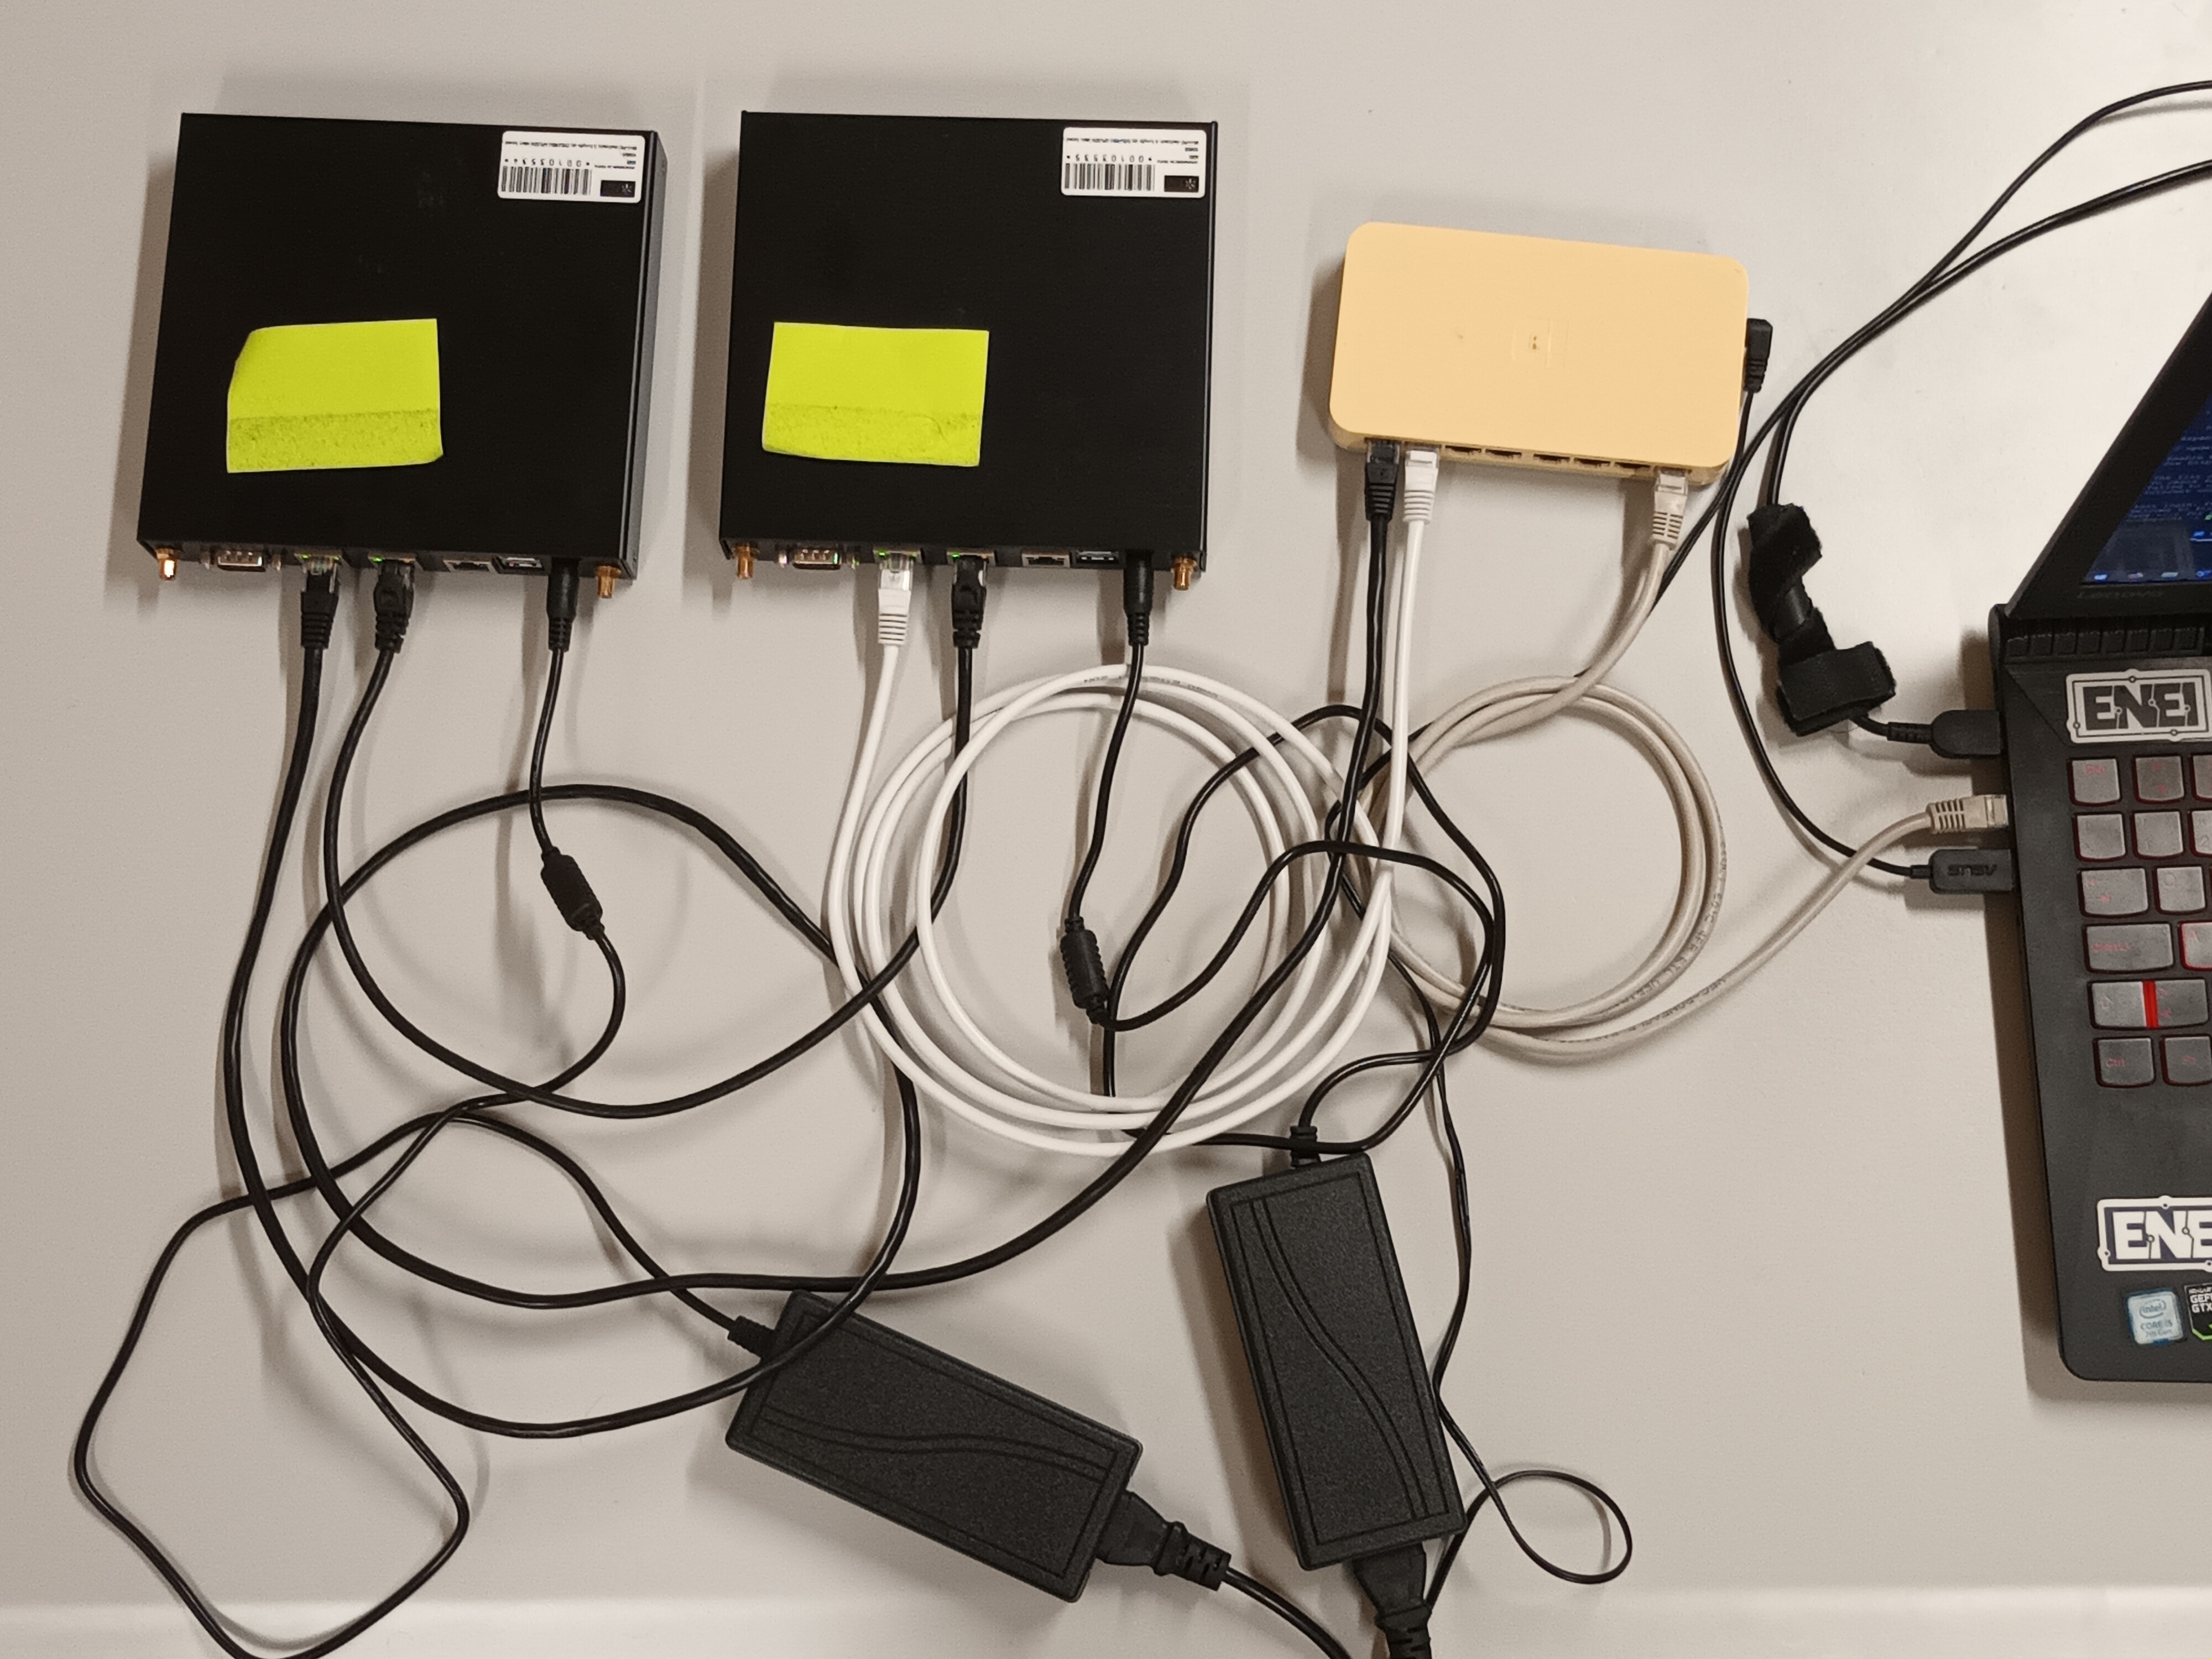
\includegraphics[width=\textwidth]{Chapters/Figures/tests/bmv2_phase_1/20241122_185833.jpg}
	\caption{Setup from the first phase of the experiments with \gls{bmv2}}
	\label{fig:exp2_phase1_setup}
\end{figure}

\begin{figure}
	\centering
	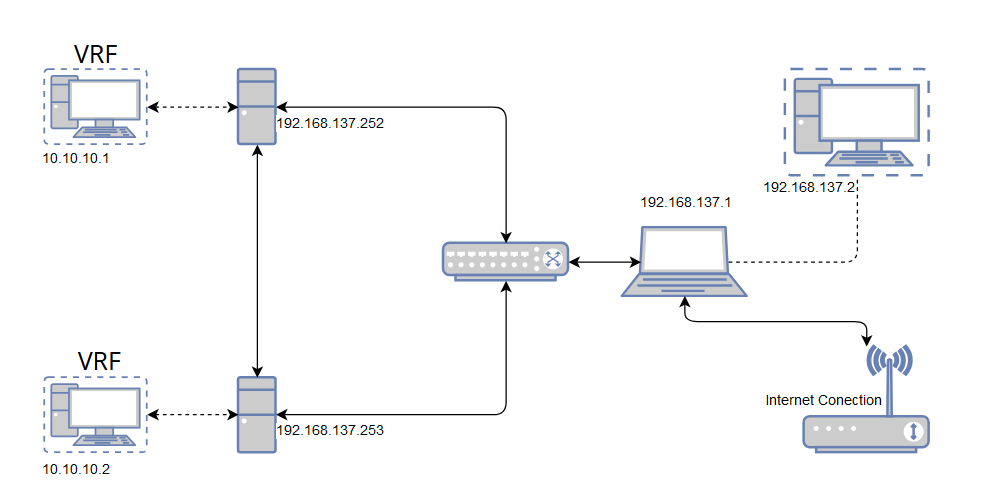
\includegraphics[width=\textwidth]{Chapters/Figures/tests/bmv2_phase_1/setup_diagram.PNG}
	\caption{Diagram that represents the setup from the first phase of the experiments with \gls{bmv2}}
	\label{fig:exp2_phase1_diagram}
\end{figure}

% Results
\subsubsection{Results}

Figure\ref{fig:exp2_phase1_bmv2} shows \gls{bmv2} running in both devices.

\begin{figure}
	\centering
	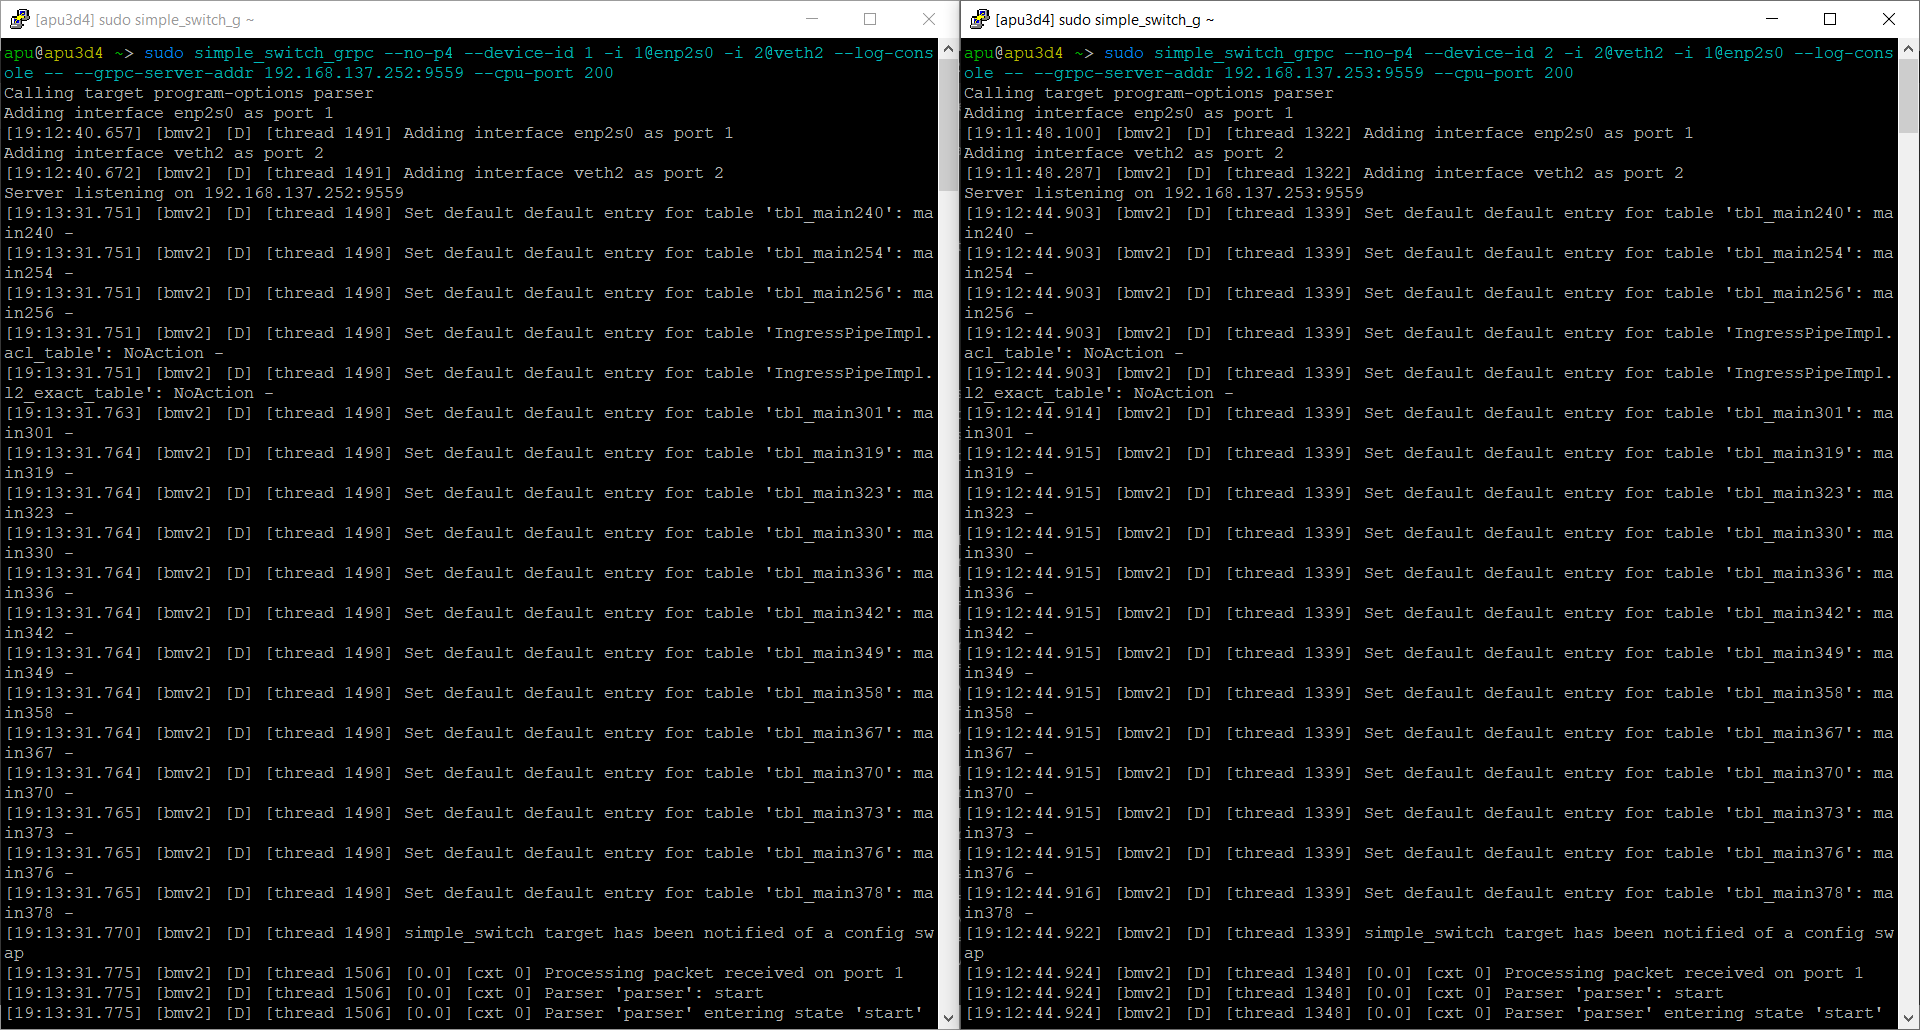
\includegraphics[width=\textwidth]{Chapters/Figures/tests/bmv2_phase_1/bmv2_running.PNG}
	\caption{Consoles running \gls{bmv2} on both devices}
	\label{fig:exp2_phase1_bmv2}
\end{figure}

Figure\ref{fig:exp2_phase1_pings} illustrates the connectivity between devices 192.168.137.252 and 192.168.137.253, manifesting through the \glspl{vrf} with \glspl{ip} 10.10.10.1 and 10.10.10.2.

\begin{figure}
	\centering
	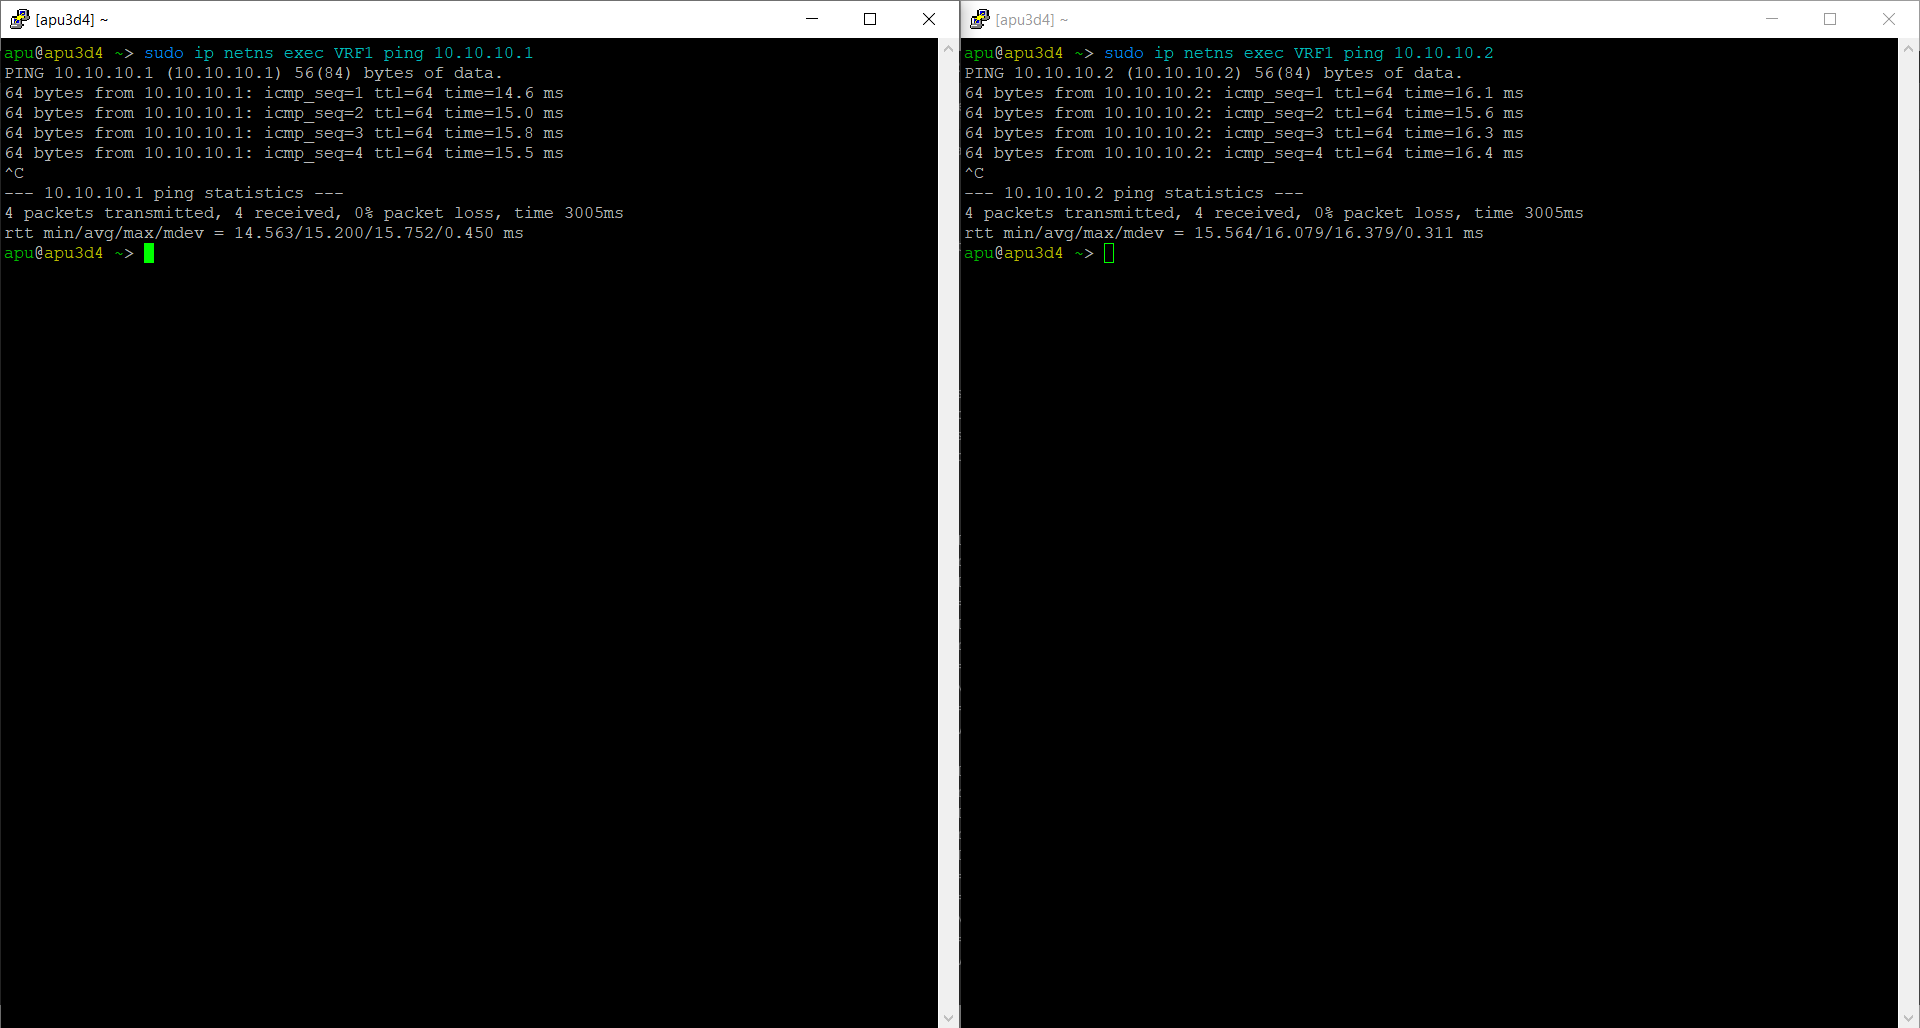
\includegraphics[width=\textwidth]{Chapters/Figures/tests/bmv2_phase_1/pings-2.PNG}
	\caption{Results from running the commands "ping" in the \gls{vrf} between the two devices on the network}
	\label{fig:exp2_phase1_pings}
\end{figure}

When viewed through the lens of \gls{sdn}, the physical configuration can be conceptualized as illustrated in Figure \ref{fig:exp2_phase1_sdn_diagram}.

\begin{figure}
	\centering
	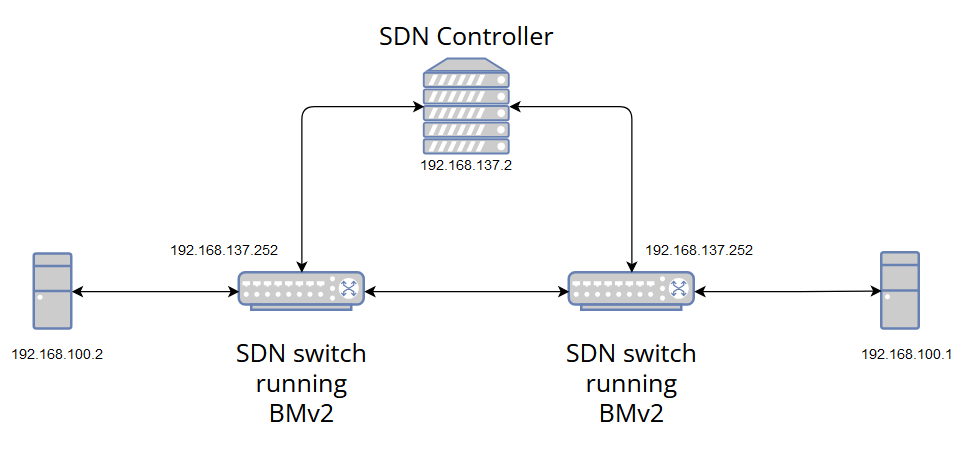
\includegraphics[width=\textwidth]{Chapters/Figures/tests/bmv2_phase_1/sdn_diagram.PNG}
	\caption{Diagram that depicts the \gls{sdn} perspective of the setup from the first phase of the experiments with \gls{bmv2}}
	\label{fig:exp2_phase1_sdn_diagram}
\end{figure}

The list of devices and hosts known to the controller is shown in Figure\ref{fig:exp2_phase1_onos}, and the flows that have been injected into the devices are presented in Figure\ref{fig:exp2_phase1_onos_flows}. The \gls{p4}/\gls{onos} application made for this phase can be seen in Figure\ref{fig:exp2_phase1_onos_apps}.

\begin{figure}
	\centering
	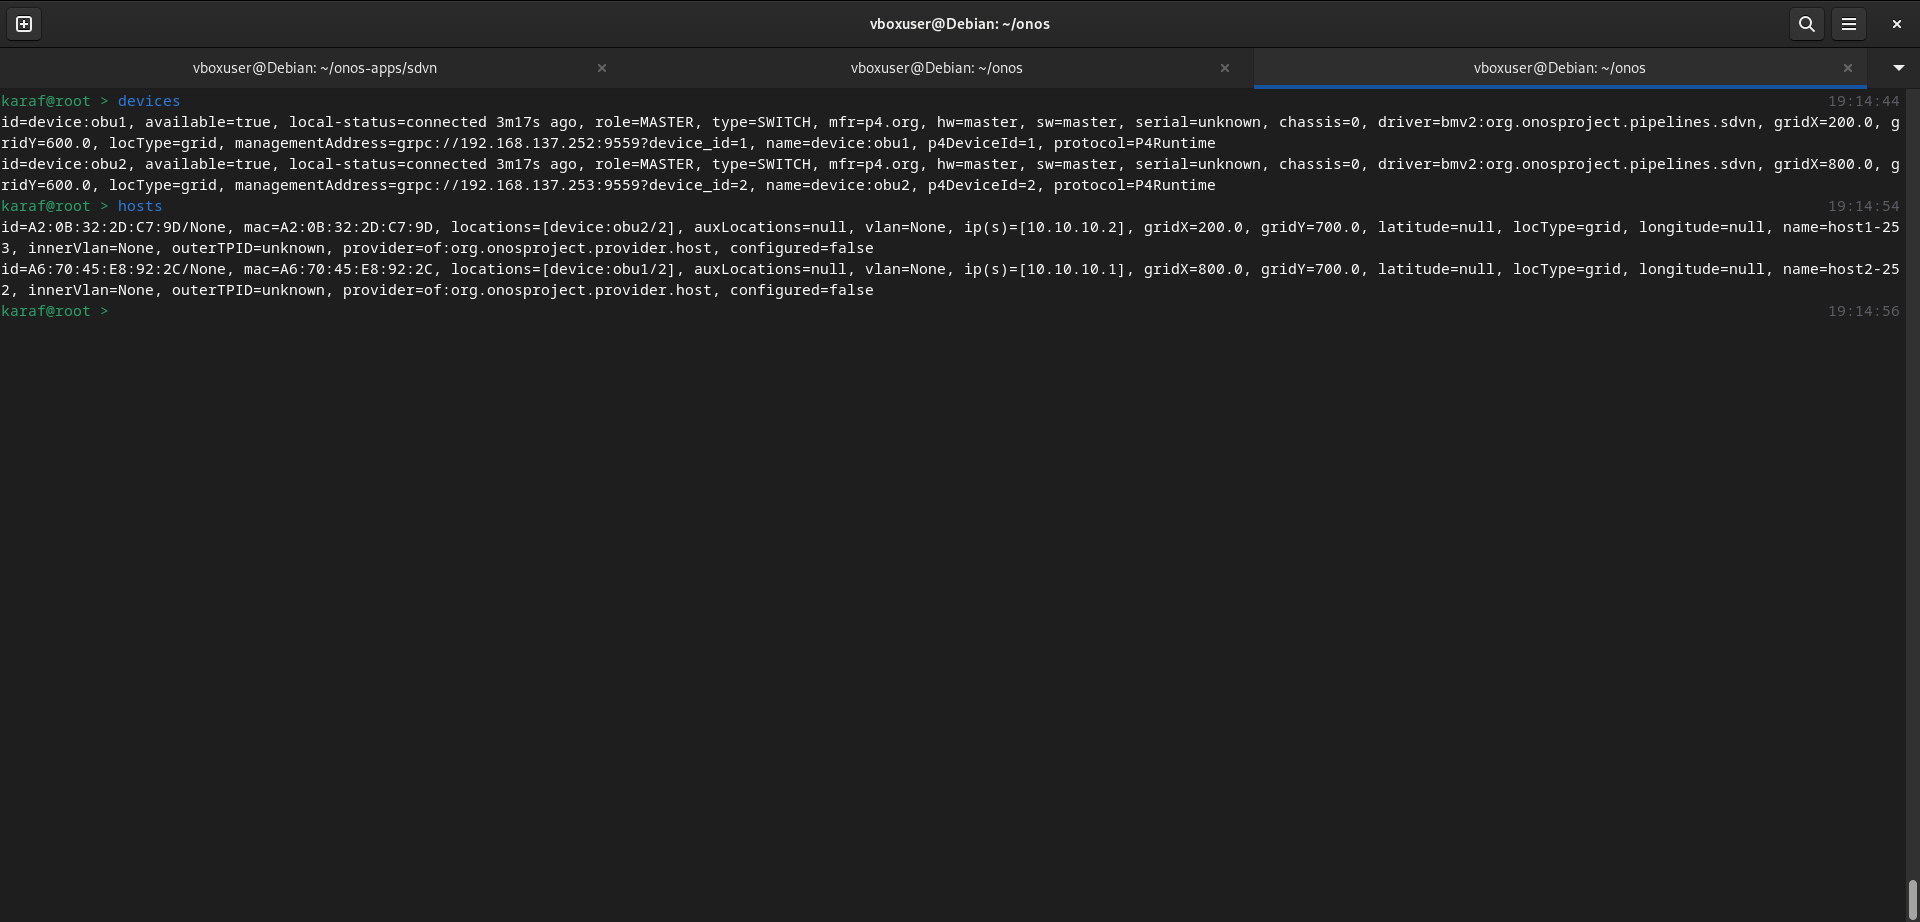
\includegraphics[width=\textwidth]{Chapters/Figures/tests/bmv2_phase_1/onos_topology.PNG}
	\caption{\gls{onos} console with information relating to the devices and hosts of the network}
	\label{fig:exp2_phase1_onos}
\end{figure}

\begin{figure}
	\centering
	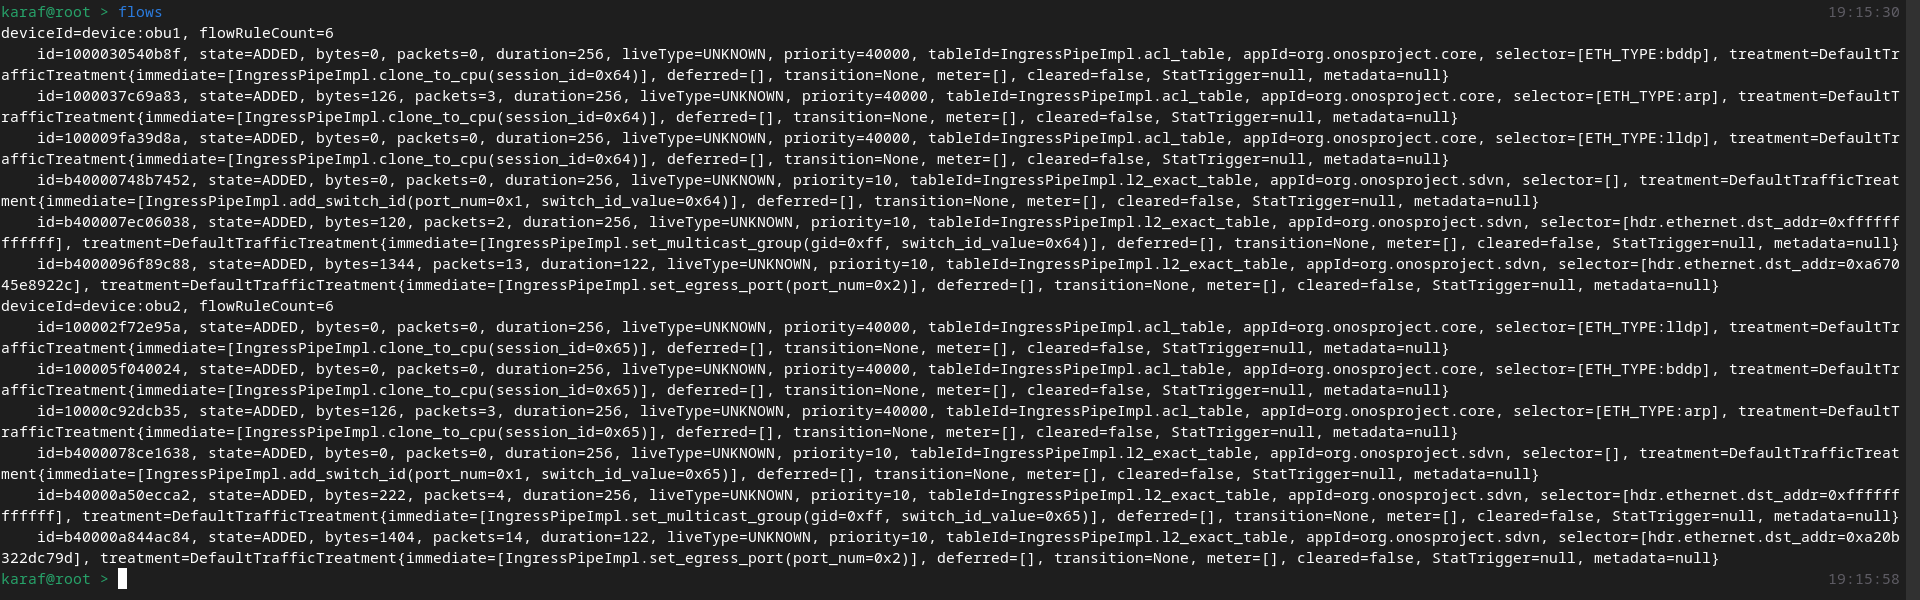
\includegraphics[width=\textwidth]{Chapters/Figures/tests/bmv2_phase_1/flows.PNG}
	\caption{\gls{onos} console with information relating to the flows of the network}
	\label{fig:exp2_phase1_onos_flows}
\end{figure}

\begin{figure}
	\centering
	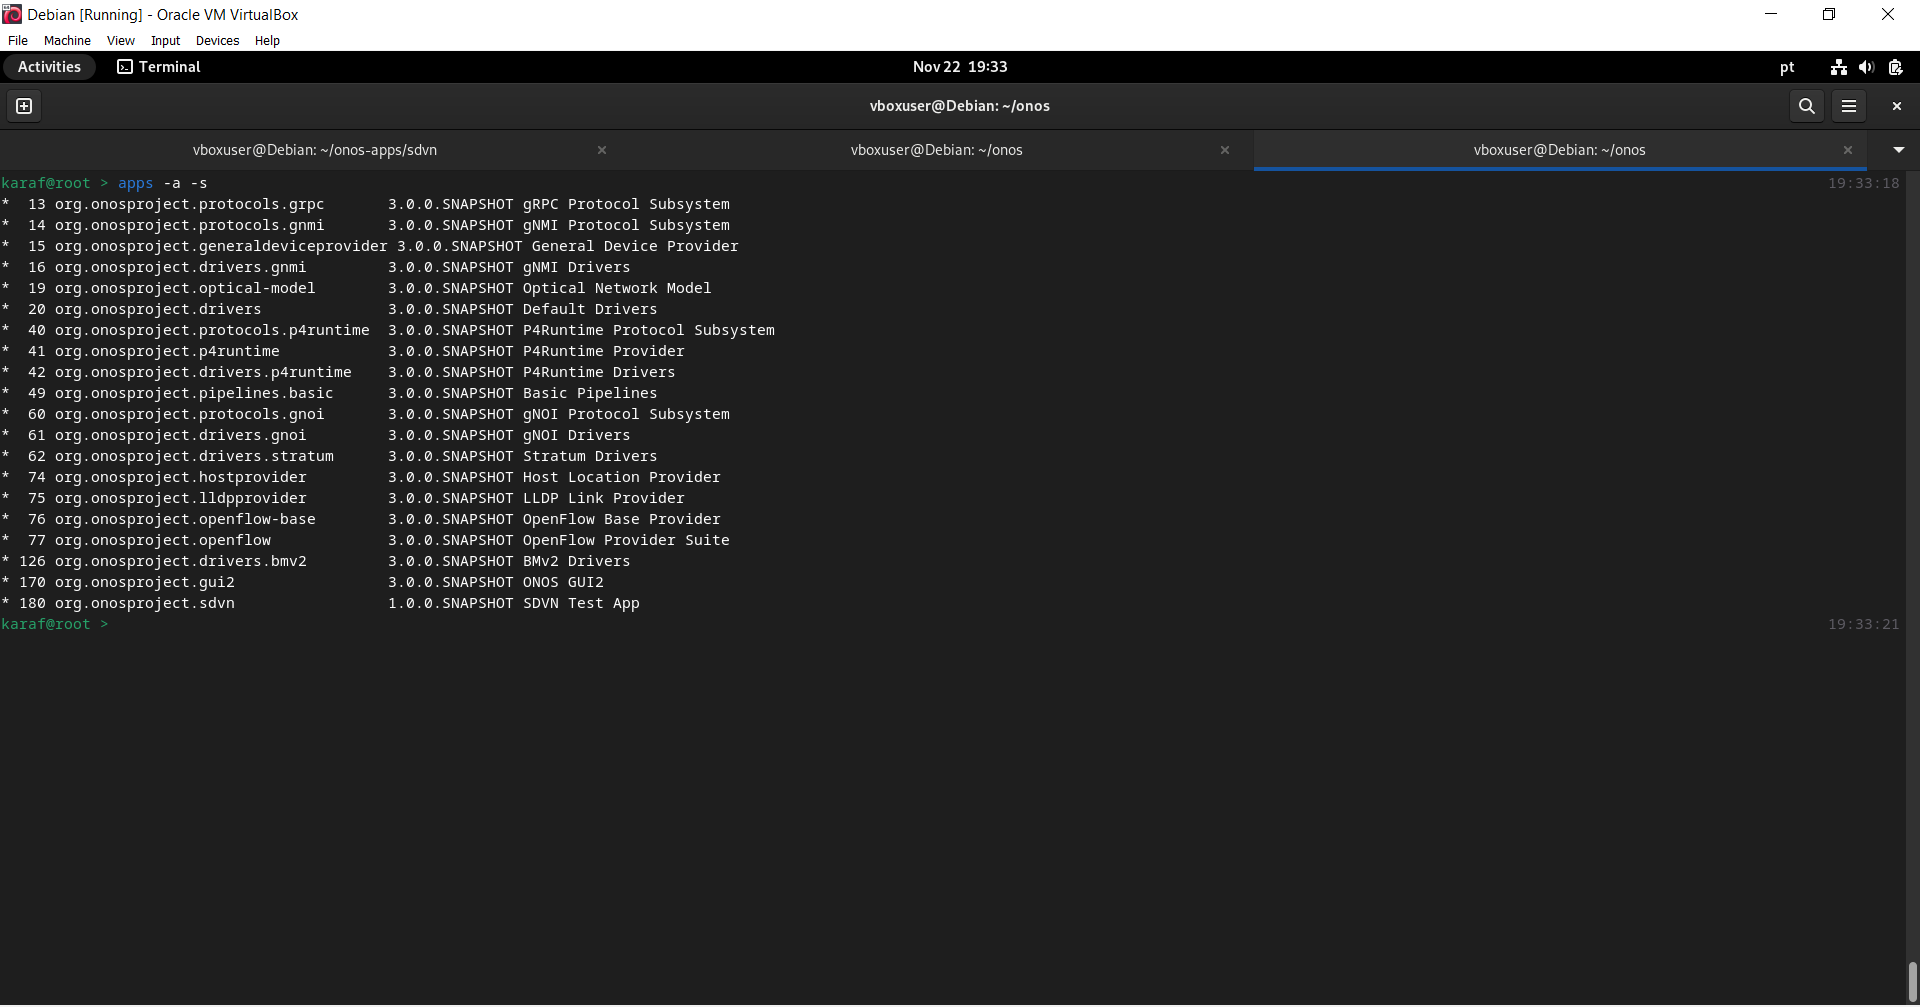
\includegraphics[width=\textwidth]{Chapters/Figures/tests/bmv2_phase_1/onos_apps.PNG}
	\caption{\gls{onos} console with information relating to the applications activated on the controller}
	\label{fig:exp2_phase1_onos_apps}
\end{figure}

% Phase 2
\subsection{Phase 2}
Phase two of the experiments with \gls{bmv2} represents a significant advancement over the initial phase, as it introduces the crucial element of wireless communication. Accordingly, the ath9k patch was implemented on the devices to enable communication at the 802.11p standard. This can be seen in Figure\ref{fig:exp2_phase2_wireless}.

\begin{figure}
	\centering
	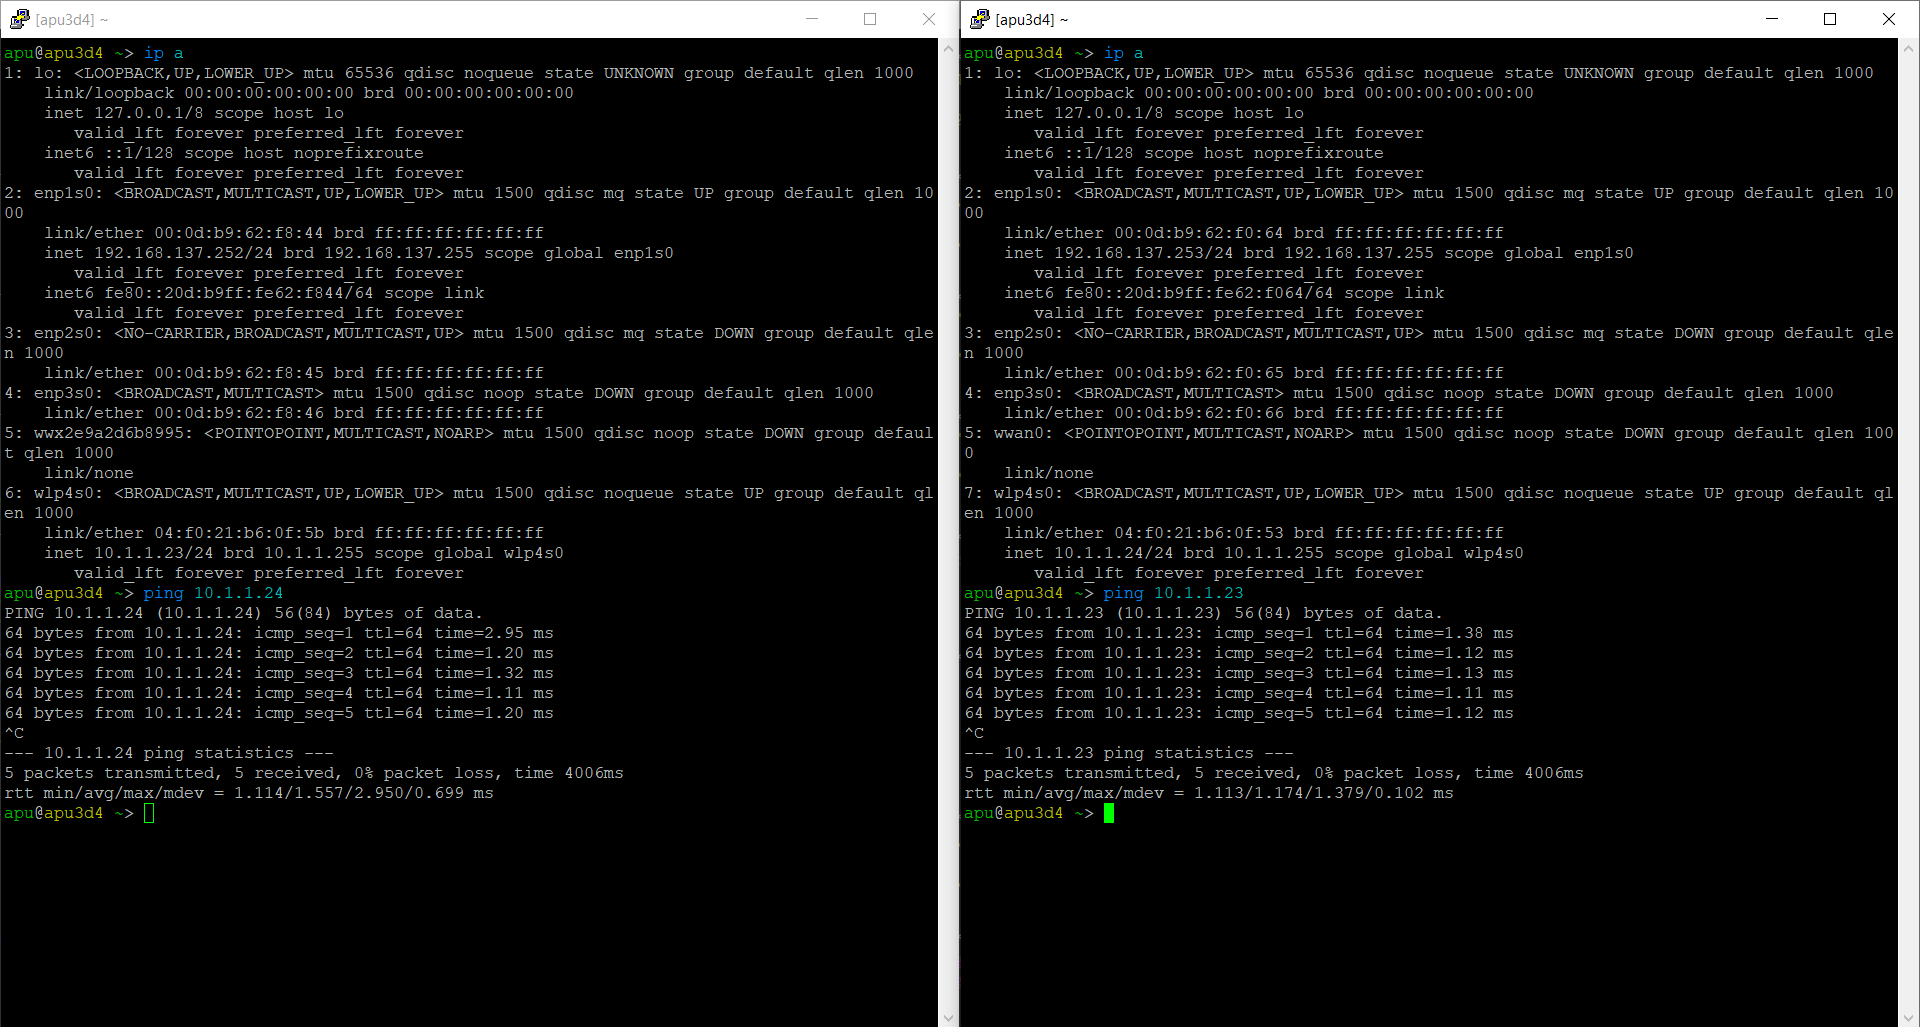
\includegraphics[width=\textwidth]{Chapters/Figures/tests/bmv2_phase_2/wireless_config_&_connectivity.PNG}
	\caption{Results from running the commands "ip a" and "ping" between the two devices on the network using the \gls{ip} address of the wireless interfaces.}
	\label{fig:exp2_phase2_wireless}
\end{figure}

As a result of this, two changes had to be made. The first of these amendments required the activation of the \gls{bmv2} with the wireless interface. The second consequence required modification of the \gls{p4}/\gls{onos} applications and configuration to accommodate the distinctive characteristics of the wireless antennas.

\begin{figure}
	\centering
	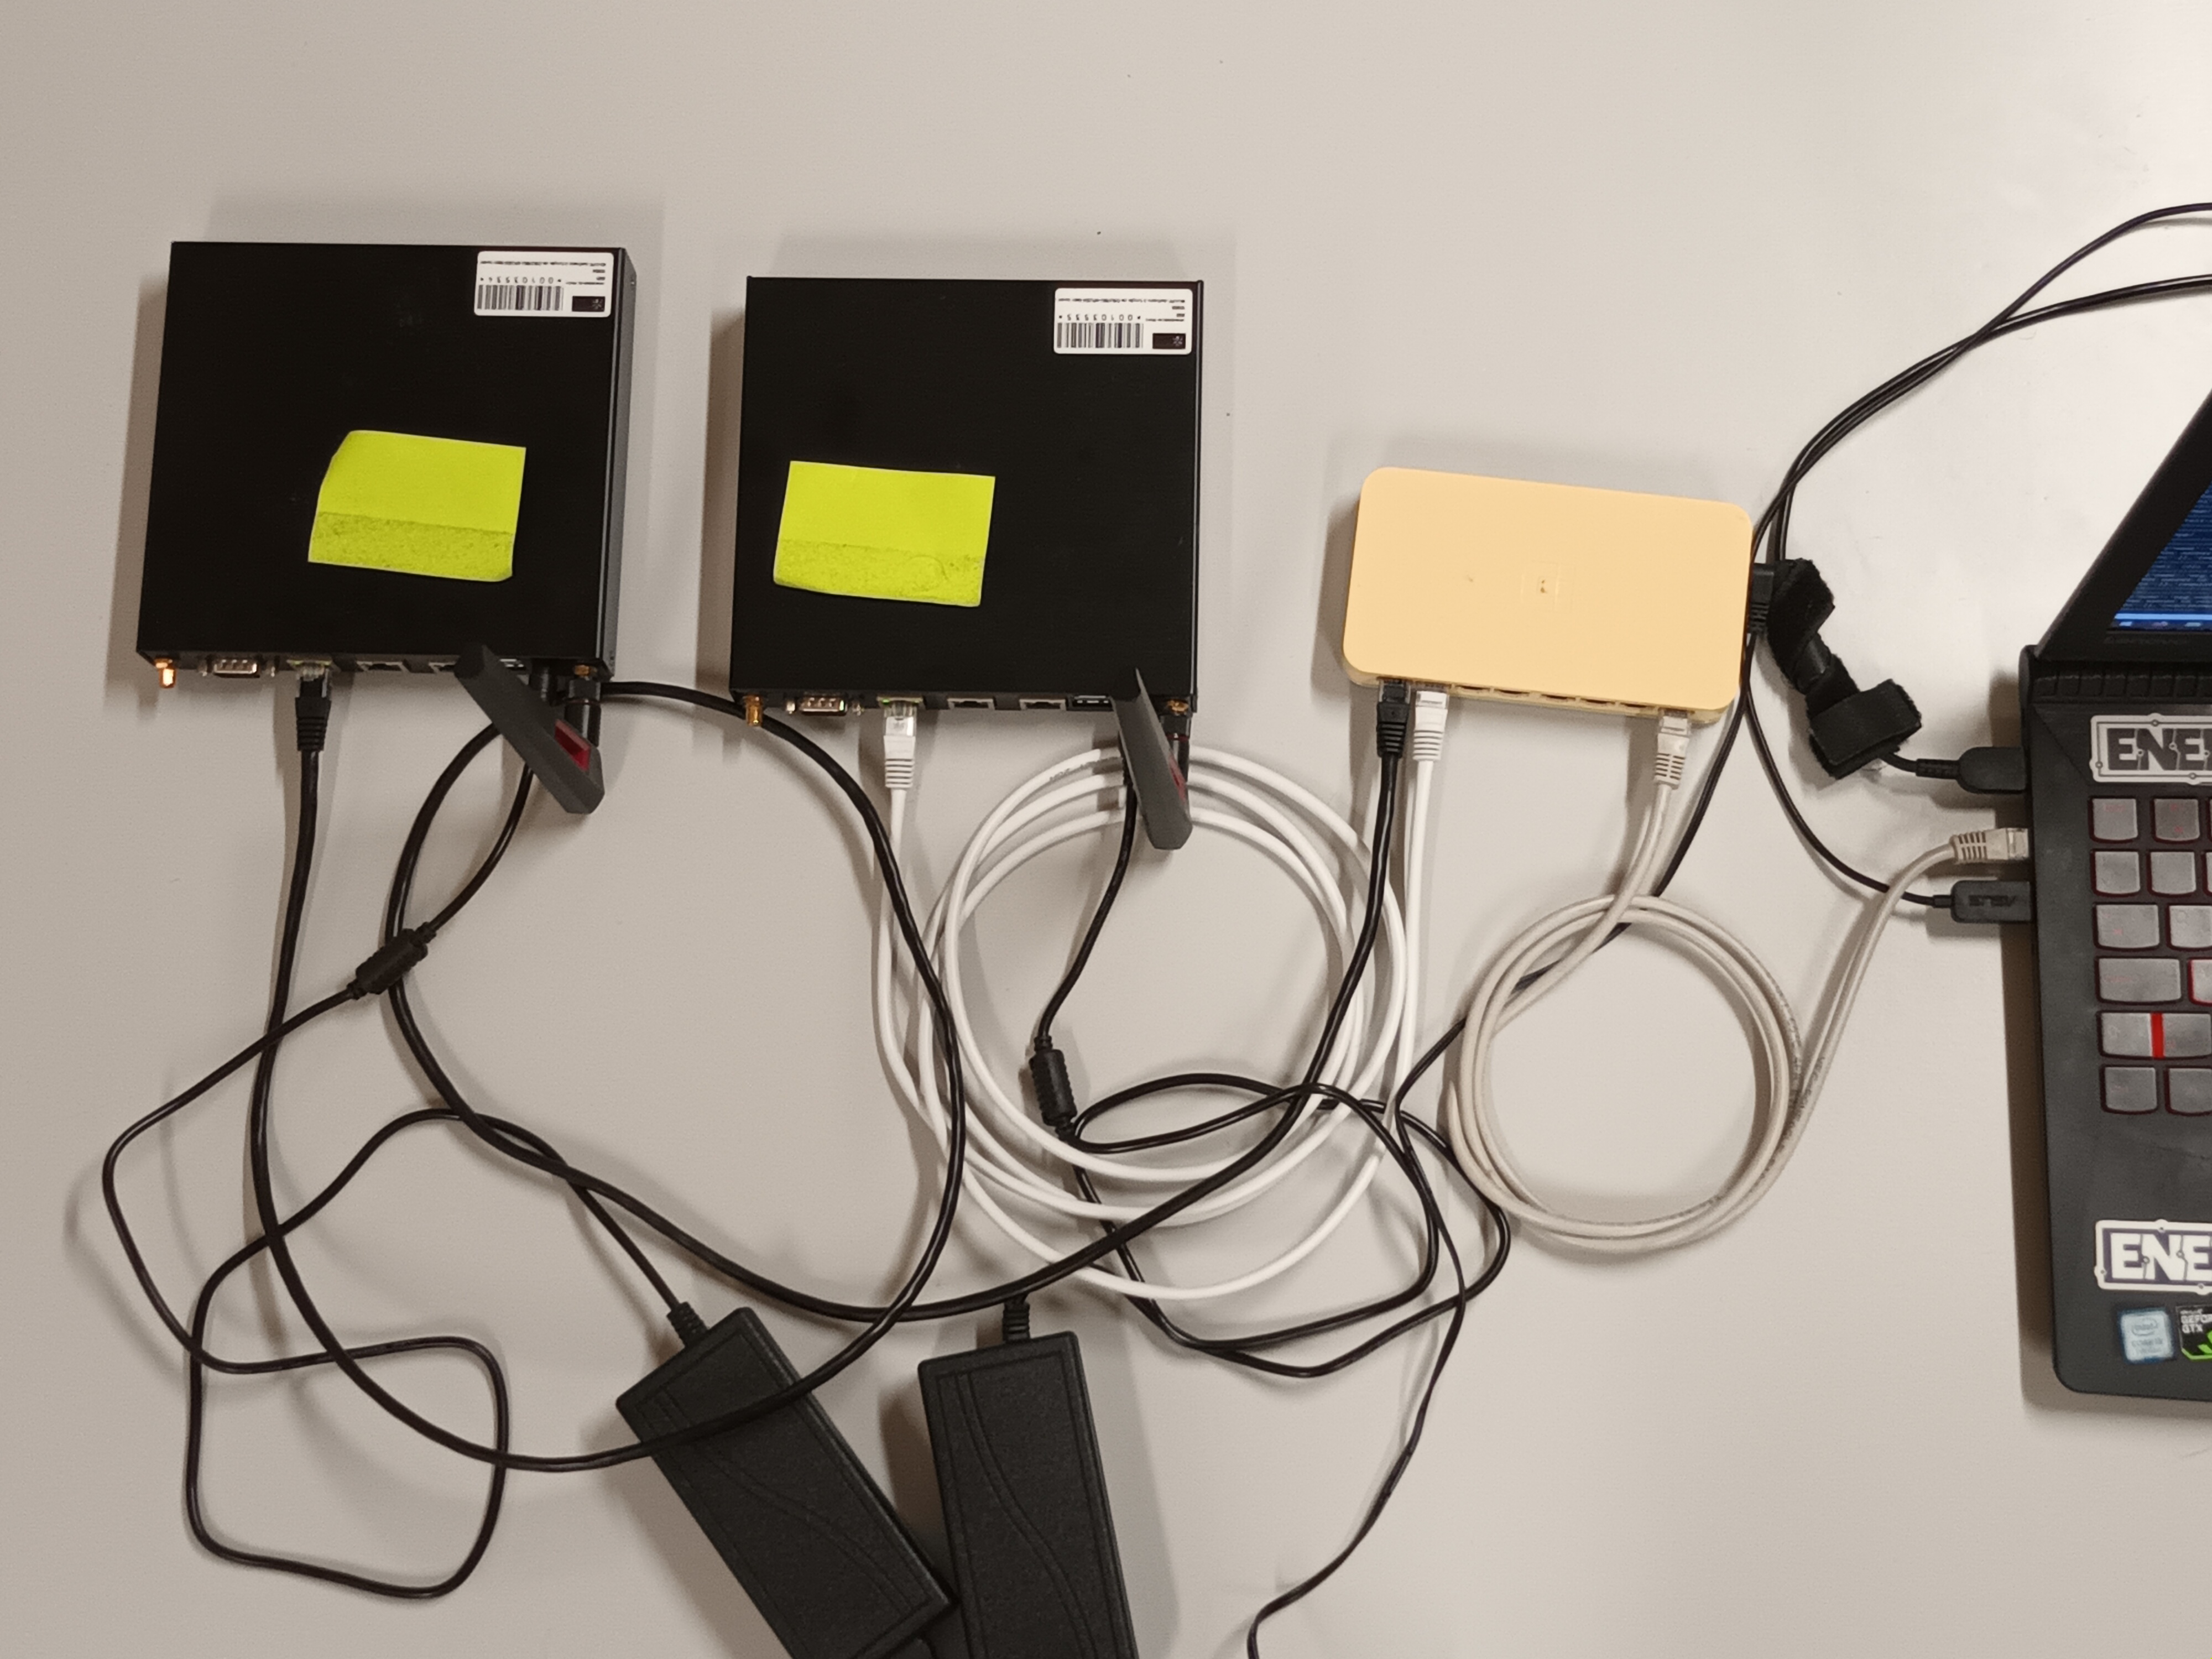
\includegraphics[width=\textwidth]{Chapters/Figures/tests/bmv2_phase_2/20241122_193213.jpg}
	\caption{Setup from the second phase of the experiments with \gls{bmv2}}
	\label{fig:exp2_phase2_setup}
\end{figure}

\begin{figure}
	\centering
	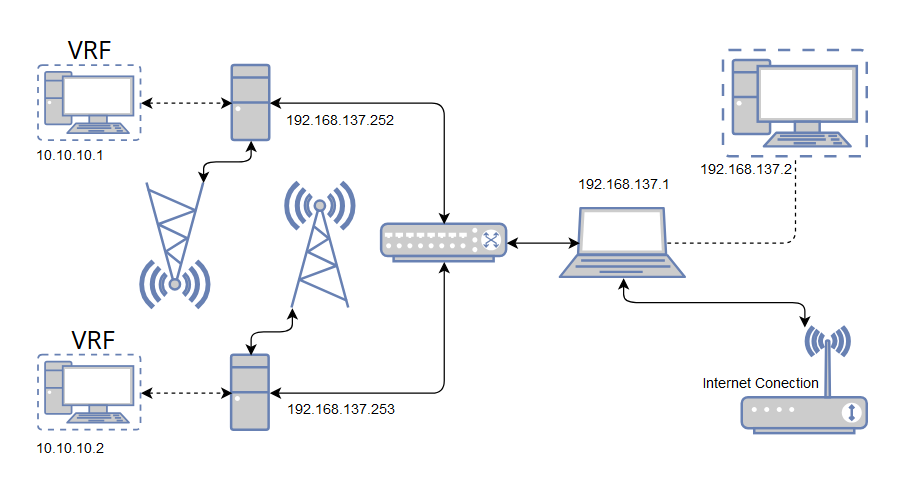
\includegraphics[width=\textwidth]{Chapters/Figures/tests/bmv2_phase_2/setup_diagram.PNG}
	\caption{Diagram that represents the setup from the second phase of the experiments with \gls{bmv2}}
	\label{fig:exp2_phase2_diagram}
\end{figure}


The test configuration is illustrated in Figure\ref{fig:exp2_phase2_setup}, which was also used as the basis for the diagram seen in Figure\ref{fig:exp2_phase2_diagram} and described in the following itemized list:

\begin{itemize}
	\item 192.168.137.1 - This \gls{ip} address identifies the author's personal laptop computer. It serves as the central coordinating hub for the entire network, facilitating the observation and monitoring of all network activity.
	\item 192.168.137.2 - This address represents a virtual machine that is hosted on the author's laptop via the Oracle VM VirtualBox virtualization platform. The virtual environment is configured with Debian 12 and is primarily intended for the deployment of \gls{onos}. This configuration is essential due to the fact that the primary branch of \gls{onos} is designed to run on Linux, whereas the author's device runs on Windows.
	\item 192.168.137.252 - This device corresponds to the version 2 of the devices. The device has a fresh installation of the Ubuntu Server operating system and is running \gls{bmv2} with grpc. Furthermore, the device is equipped with an antenna capable of communicating at frequencies up to 6 GHz and has been applied with the ath9k patch to the WiFi driver, thereby enabling communication using 802.11p.
	\item 192.168.137.253 - This device is virtually identical to the device 192.168.137.252.
	\item 10.10.10.1 - This \gls{ip} address identifies the virtual interface that has been added to the \gls{vrf} instance created in the 192.168.137.252 device.
	\item 10.10.10.2 - Identically to the last one, this \gls{ip} address identifies the virtual interface that has been added to the \gls{vrf} instance created in the 192.168.137.253 device.
\end{itemize}

% Results
\subsubsection{Results}


Figure\ref{fig:exp2_phase2_bmv2} shows \gls{bmv2} running in both devices.

\begin{figure}
	\centering
	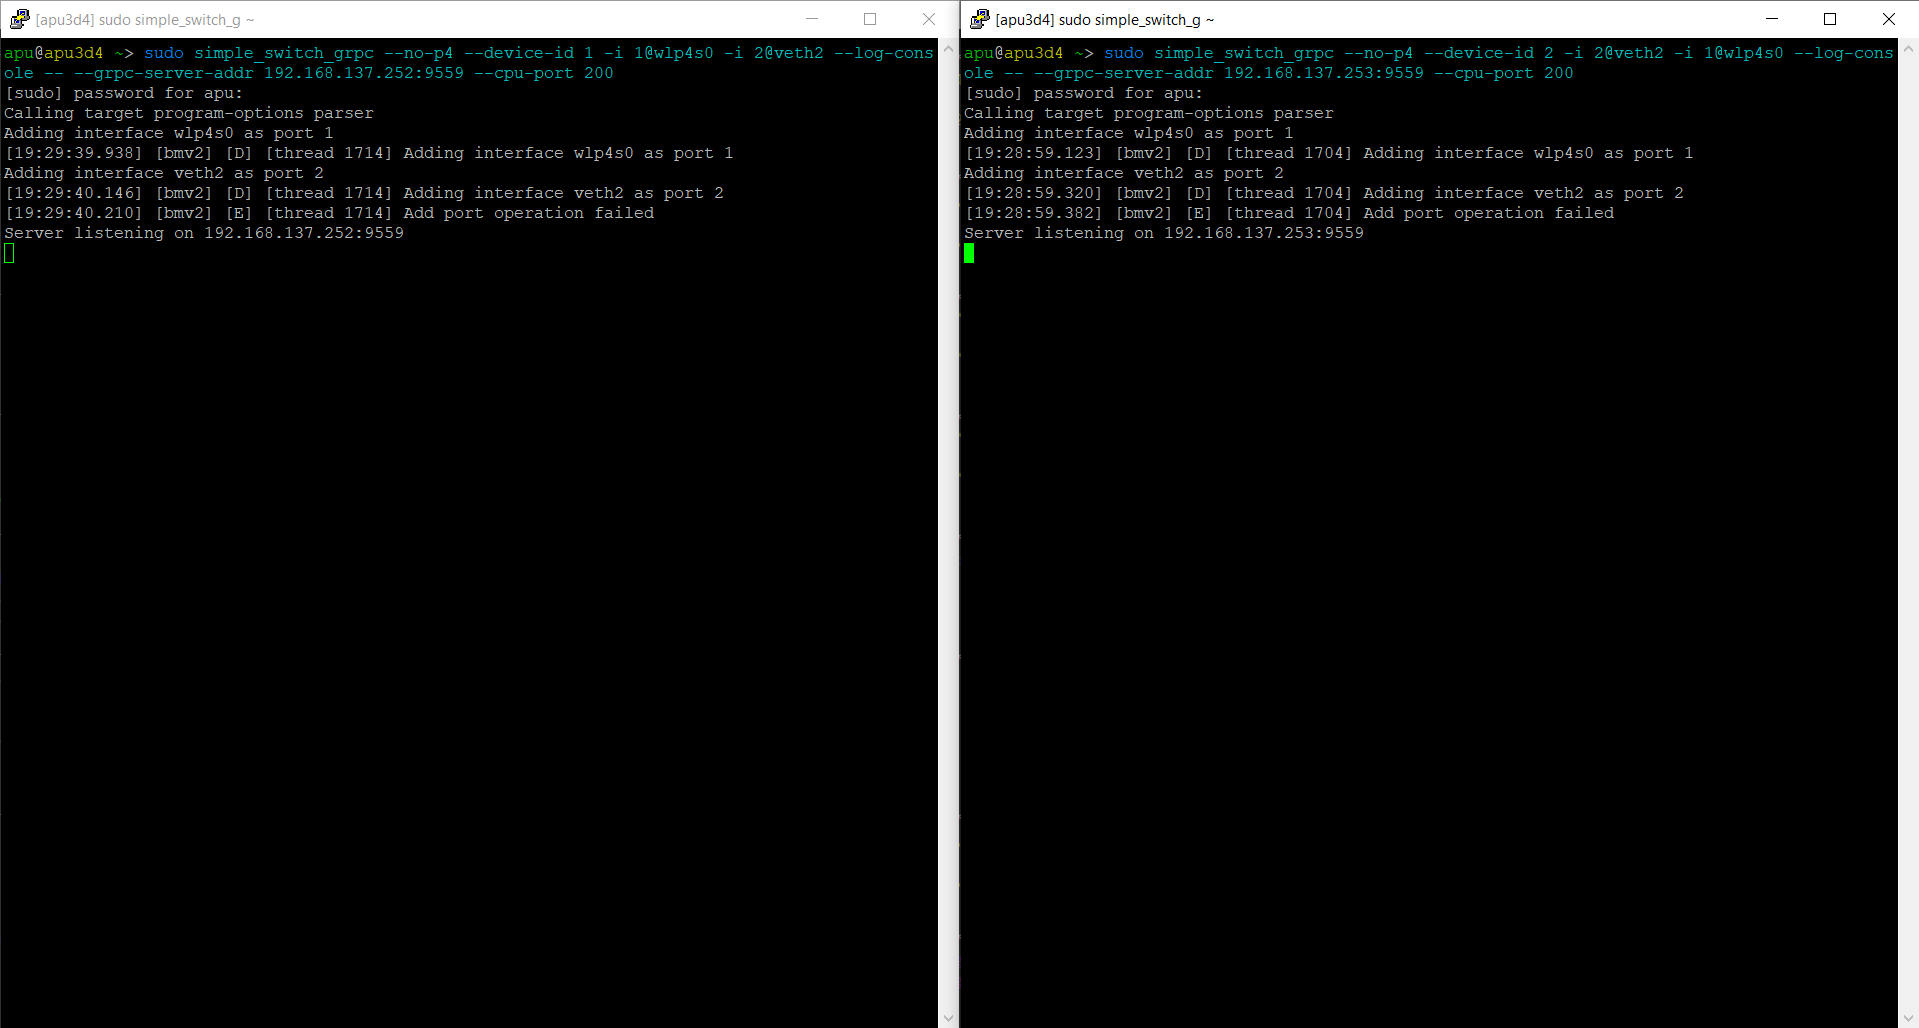
\includegraphics[width=\textwidth]{Chapters/Figures/tests/bmv2_phase_2/bmv2_running.PNG}
	\caption{Consoles running \gls{bmv2} on both devices}
	\label{fig:exp2_phase2_bmv2}
\end{figure}

Figure\ref{fig:exp2_phase2_pings} illustrates the connectivity between devices 192.168.137.252 and 192.168.137.253, manifesting through the VFRs with \glspl{ip} 10.10.10.1 and 10.10.10.2.

\begin{figure}
	\centering
	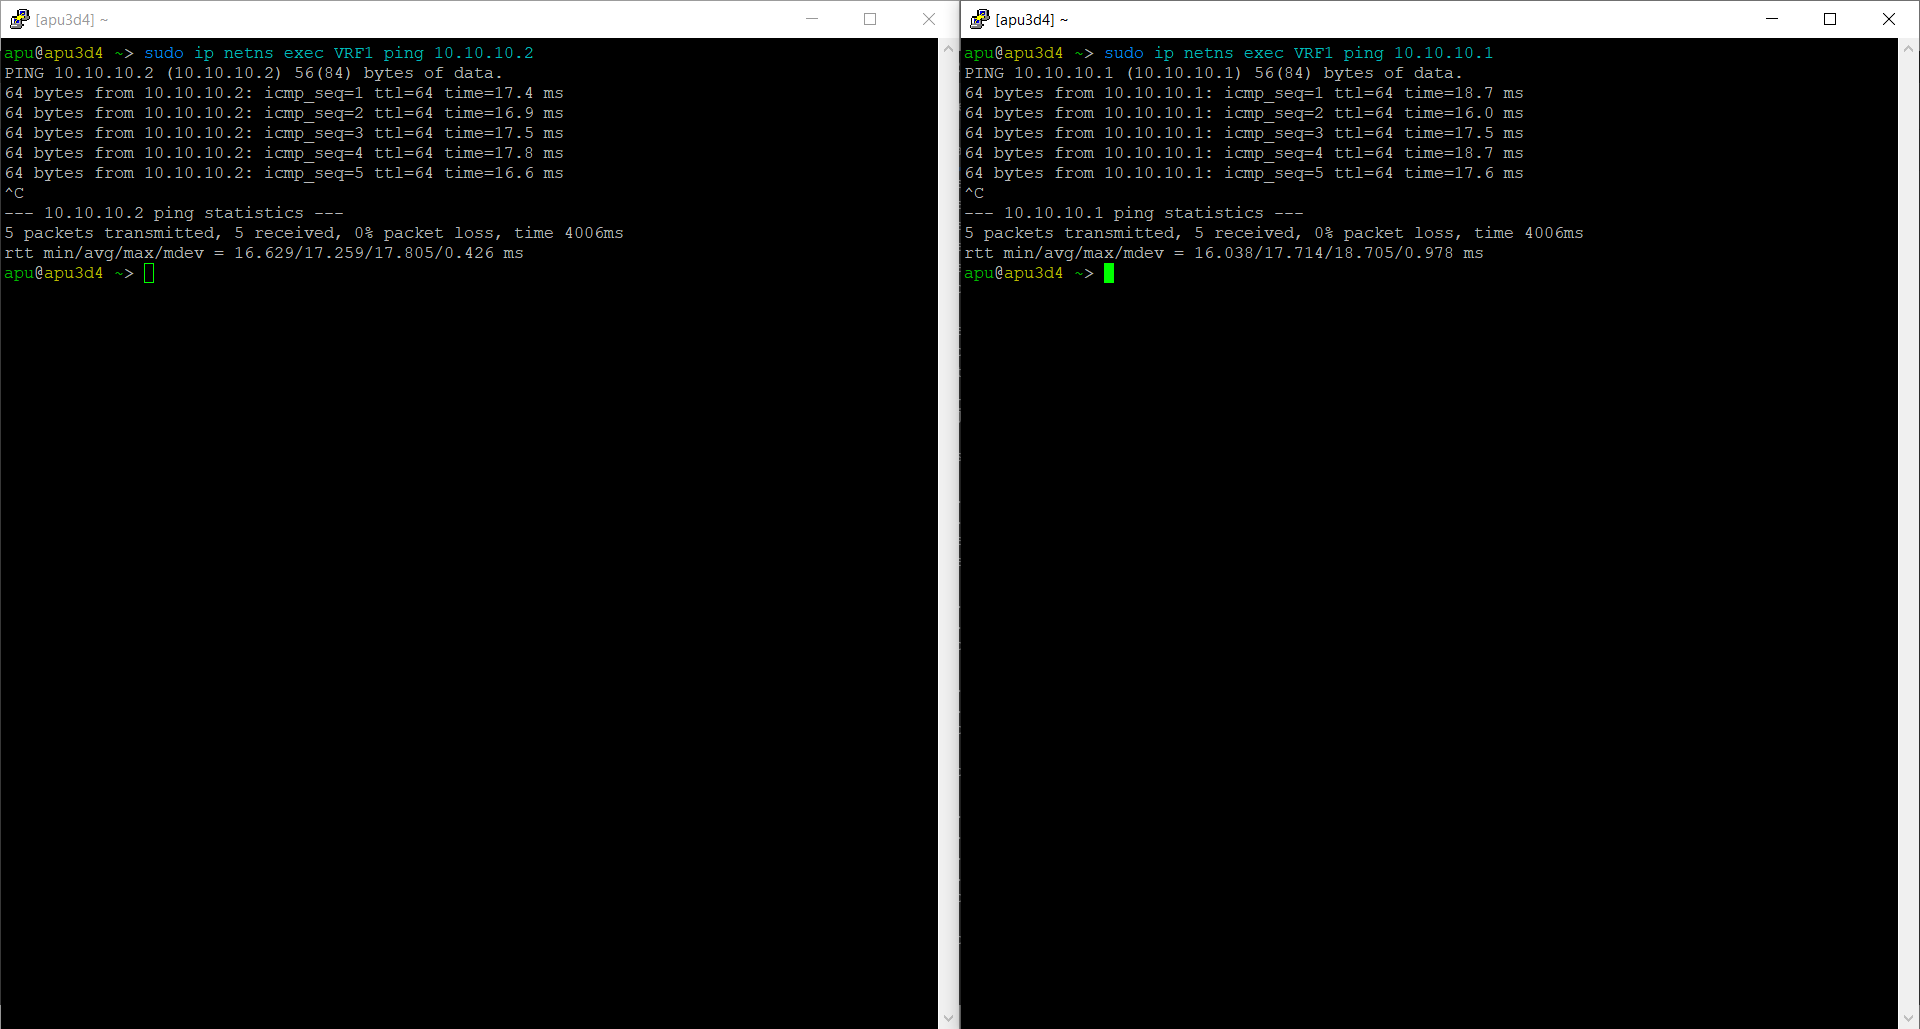
\includegraphics[width=\textwidth]{Chapters/Figures/tests/bmv2_phase_2/pings.PNG}
	\caption{Results from running the commands "ping" in the \gls{vrf} of the two devices on the network}
	\label{fig:exp2_phase2_pings}
\end{figure}

In order for communication to be established between the devices, it was necessary to make modifications to the program created in the first phase. For any message to be successfully received by an antenna, that antenna's destination Media Access Control address must either be the address of the antenna or the broadcast address. It was thus decided to pursue the latter course of action, which entailed changing the addresses of the messages sent via the wireless interface to the broadcast address. The original address is stored within the packet and inserted when required.

When viewed through the lens of \gls{sdn}, the physical configuration can be conceptualized as illustrated in Figure\ref{fig:exp2_phase2_sdn_diagram}.

\begin{figure}
	\centering
	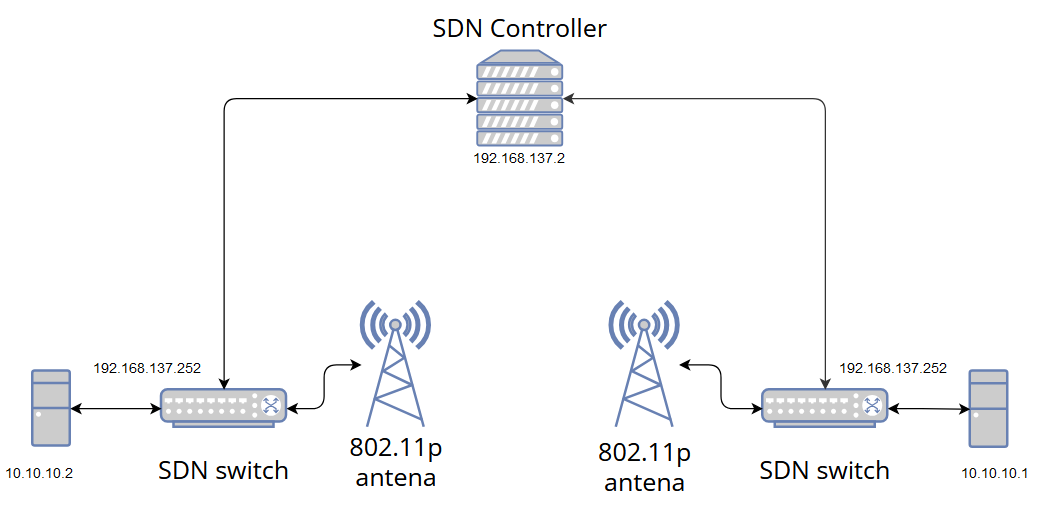
\includegraphics[width=\textwidth]{Chapters/Figures/tests/bmv2_phase_2/sdn_diagram.PNG}
	\caption{Diagram that depicts the \gls{sdn} perspective of the setup from the second phase of the experiments with \gls{bmv2}}
	\label{fig:exp2_phase2_sdn_diagram}
\end{figure}


The list of devices and hosts known to the controller is shown in Figure\ref{fig:exp2_phase2_onos}, and the flows that have been injected into the devices are presented in Figure\ref{fig:exp2_phase2_onos_flows}.

\begin{figure}
	\centering
	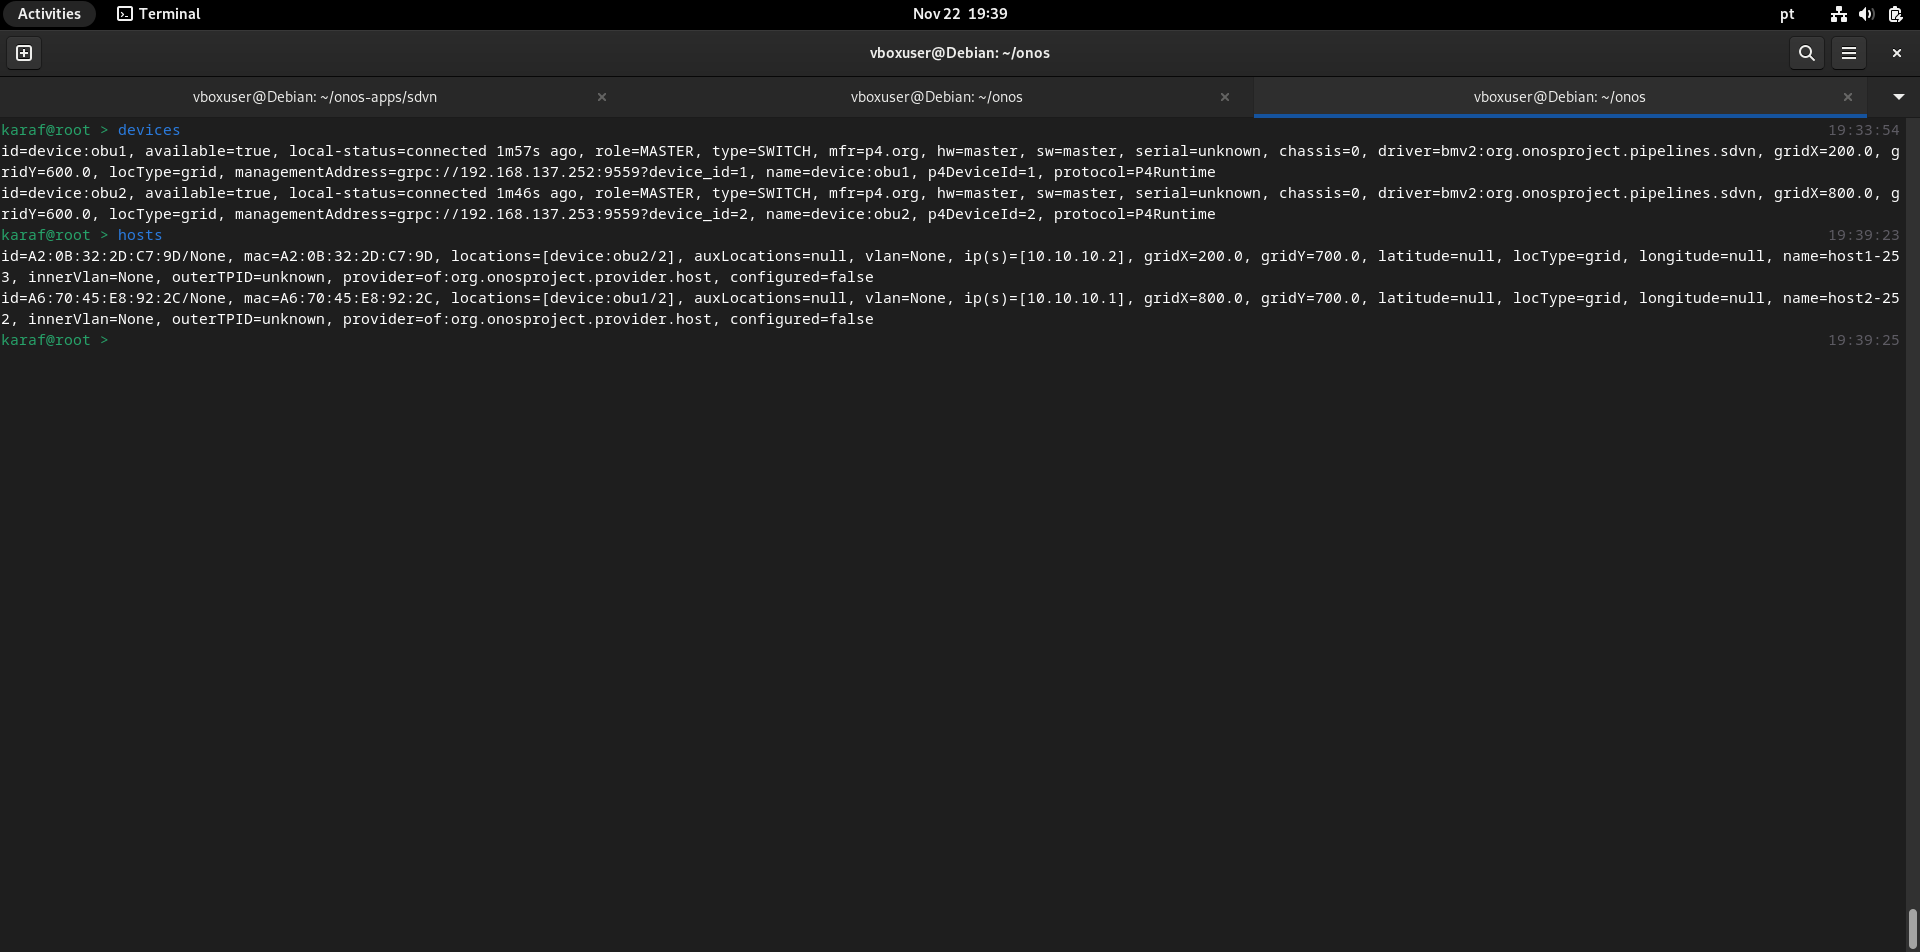
\includegraphics[width=\textwidth]{Chapters/Figures/tests/bmv2_phase_2/onos_topology.PNG}
	\caption{\gls{onos} console with information relating to the devices and hosts of the network}
	\label{fig:exp2_phase2_onos}
\end{figure}

\begin{figure}
	\centering
	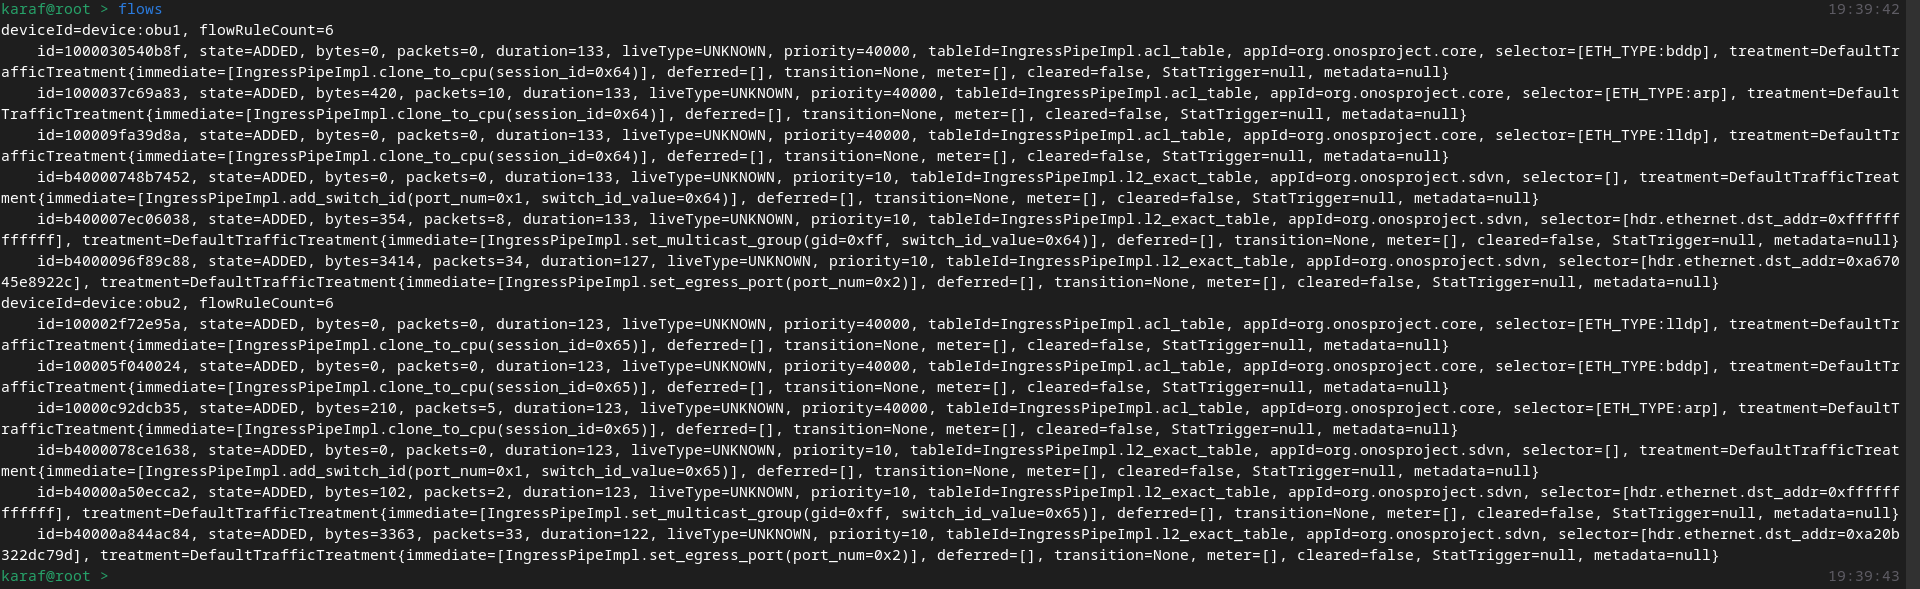
\includegraphics[width=\textwidth]{Chapters/Figures/tests/bmv2_phase_2/onos_flows.PNG}
	\caption{\gls{onos} console with information relating to the flows of the network}
	\label{fig:exp2_phase2_onos_flows}
\end{figure}

% Limitations
\subsection{Limitations}
This experiment was constrained by a significant limitation, namely the availability of only two devices with \gls{bmv2} installed for use. As previously stated, the original device provided by the university is not suitable for use in this scenario due to insufficient storage capacity to install \gls{bmv2}. Furthermore, financial constraints precluded the acquisition of another device of the newer version.
Obtaining more than two devices was crucial to effectively recreate more intricate testing scenarios that more closely resemble real-world contexts, such as the transmission of a message through a network of wireless devices. However, despite the inability to demonstrate this specific scenario due to a lack of resources, the observed functionality of the program, its code, and the logs from \gls{bmv2} and \gls{onos} provide strong indications that the code will perform as intended in the aforementioned scenario. Nevertheless, tests of this nature are regrettably not feasible at this time.

% Analysis and Interpretation
\subsection{Analysis and Interpretation}
In Phase 1 of these tests, it was an unanticipated finding that the default southbound \gls{api} of \gls{bmv2} is not P4Runtime, as had been previously assumed, but rather Thrift. The Thrift \gls{api}\cite{noauthor_apache_nodate} is a component of the Apache Thrift framework, which originated at Facebook. The goal of Thrift is to facilitate cross-language communication and data serialization by providing a language-agnostic interface that can be implemented in a variety of programming languages. In this case, Thrift is used to turn an easy to read file with controller instructions to device specific instruction in the data plane.

This decision by the developers may initially seem incongruous, but it is, in fact, a logical consequence of the broader strategic context. \gls{bmv2} is not a production-grade switch; rather, it is a software tool designed for educational and experimental purposes in conjunction with \gls{p4}. Thrift offers a more straightforward mechanism that streamlines the process of inserting rules on network devices. 
In consideration of this fact, it is clear that \gls{bmv2} was not developed with high performance as a primary objective. Accordingly, any practical development should seek to implement a faster solution in the event that performance issues arise.

The transposition of the final scenario to an \gls{sdn} network, which was illustrated in Figure\ref{fig:exp2_phase2_sdn_diagram}, to an Vehicle \gls{its} sub-system has resulted in the diagram presented in Figure\ref{fig:exp2_vehicle_subsystem}. From this diagram, a number of interesting observations and comparisons can be made. 
In this context, the \gls{sdn} switch can be compared to an \gls{its-s} gateway and an \gls{its-s} router. It is clear that any comparison should be viewed with caution, as the device under consideration does not align perfectly with any of the aforementioned categories. This comparison is intended to illustrate the device's functionality, rather than to provide a definitive categorization. It is inaccurate to categorize this device as an \gls{osi} stack to \gls{etsi} protocol translator, as it lacks the requisite functionality to perform such a translation.
The \gls{sdn} controller could be integrated into the vehicle \gls{its} station as an \gls{its} application in a manner that would align with the standards and classifications set forth by the \gls{etsi}.

\begin{figure}
	\centering
	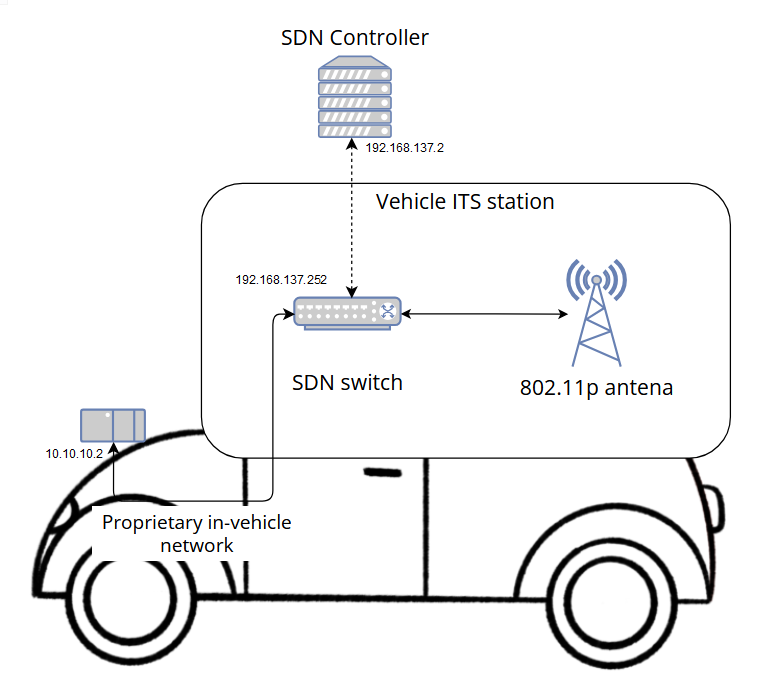
\includegraphics[width=\textwidth]{Chapters/Figures/tests/bmv2_phase_2/its_vehicle_diagram.PNG}
	\caption{Diagram representing the \gls{sdn} network as an Vehicle \gls{its} sub-system}
	\label{fig:exp2_vehicle_subsystem}
\end{figure}

As anticipated, the \gls{bmv2} proved to be the optimal choice. This experiment was successful in enabling \gls{bmv2} to function with an \gls{onos} controller and the ath9k patch. The development of this test demonstrates that \gls{p4} is capable of functioning with 802.11p, which indicates that this technology can be utilized for vehicular deployment. The power and control provided by \gls{p4} affords users a vast array of potential applications. With it and according to our tests it is possible to create a \gls{p4} based network that complies with \gls{etsi} norms, making it possible for this technology to be used in the real world.

